\chapter{Ising Model}\label{chap:ising}
%


\begin{figure}[h]
\begin{center}
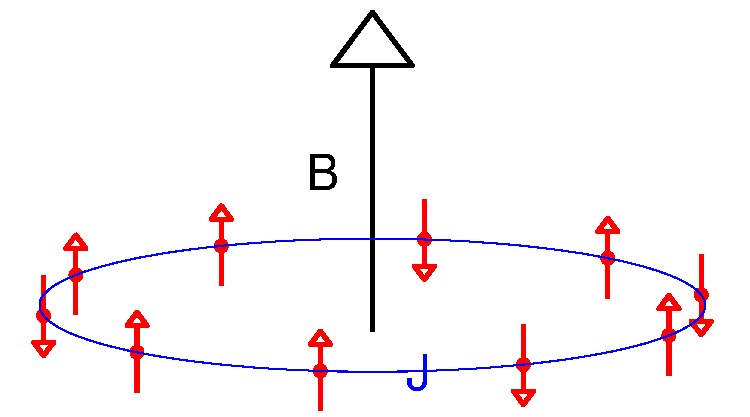
\includegraphics[width=5.5cm]{ising_spins}
\caption{{\it Arrangement of Ising-spins in a 1d chain with pbc.}}
\end{center}
\end{figure}
%



We will now examine collective magnetism.
The simplest model for this purpose is the Ising model, which is described by the following
Hamilton function 
%
\begin{align}
H &= - J \sum_{\langle i,j\rangle} S_{i} S_{j} - B \hat M\\
\text{with} \qquad \hat M &=  \mu \sum_{i} S_{i}\;,\qquad \bigg(\mu := - \frac{\mu_{B} g_{e}}{2}\bigg)\\
H&= - J \sum_{\langle i,j\rangle} S_{i} S_{j} - \mu B \sum_{i} S_{i}\;,
\end{align}
%
where the spins $S_{i}$ can only take the values  $S_{i}=\pm 1$.
$\mu_{B}$ is the Bohr magneton and $g_{e}$ the electronic Land\'e factor.
$J$ is the exchange coupling and the sum over sites is restricted to nearest neighbour sites, \red{such that each neighbouring pair is only counted once!}
$B$ stands for the magnetic flux density.
The Ising model is also used to describe binary alloys.
However, the parameters then have a different meaning.
The Ising model can be solved exactly in 1d and 2d and in $2d$ it even has a phase transition. 
We consider periodic boundary conditions \footnote{In most cases, boundary conditions are 
irrelevant in the  thermodynamic limits. } 

\section{Exact solution in 1D}
The Hamilton function of the Ising model in 1D reads
%
\begin{align*}
H &= - J \sum_{i=1}^{N} S_{i} S_{i+1} - \mu  B \frac{1}{2} \sum_{i} (S_{i}+S_{i+1})\\
\text{(pbc):}\qquad S_{i+N} &= S_{i}\;.
\end{align*}
%

\subsubsection{Canonical partition function}

The evaluation is particularly simply in the canonical ensemble:
\begin{align*}
Z(T,N,B) &= \sum_{\{S_{i}\}=\pm 1}\; e^{\beta J \sum_{ i} S_{i }S_{i+1} + \frac{\mu\beta B}{2} \sum_{i} (S_{i}+S_{i+1})}\\
 &= \sum_{\{S_{i}\}=\pm 1}\;
 \prod_{i=1}^{N}
  e^{j  S_{i }S_{i+1} + \frac{b}{2} (S_{i}+S_{i+1})}\;.
\end{align*}
%
We introduced the abbreviations $j = \beta J$ for the exchange coupling and $b = \mu B \beta$ for the magnetic flux density.
We also define the 
{\bf transfer matrix}
%
\begin{subequations}\label{eq:transfer:1d}
\begin{align}
{\cal T}_{s,s'} &:=   e^{j \; s s' + \frac{b}{2} (s + s')}\\
%
\text{which has the  matrix elements}\qquad
{\cal T}_{s,s'}&=
\begin{tabular}{c|ccc}   & +1 & -1 \\\hline+1 & $e^{j+b}$ & $e^{-j}$  \\-1 & $e^{-j}$ & $e^{j-b}$
\end{tabular}\\
%
\text{then:}\qquad Z(T,N,B)&= \sum_{\{S_{i}\}=\pm 1}\;
 \prod_{i=1}^{N} {\cal T}_{S_{i},S_{i+1}}\;.
\end{align}
\end{subequations}
%
We first consider the case $N=2$, where the partition function reads
%
\begin{align*}
Z(T,N=2,B) &= \sum_{S_{1}=\pm 1}\sum_{S_{2}=\pm 1}\;
{\cal T}_{s_{1},s_{2}}\;{\cal T}_{s_{2},s_{1}} = \sum_{s_{1}} \big({\cal T}^{2}\big)_{s_{1},s_{1}} = \tr{{\cal T}^{2}}
\end{align*}
%

The generalization to $N>2$ leads  obviously to
%
\begin{align*}
Z(T,N,B) &= \tr{{\cal T}^{N}}\;.
\end{align*}
%
The transfer matrix is real-symmetric and can be expressed in the spectral representation as follows
%
\begin{align*}
{\cal T} &= U D U^\dagger\;,
\end{align*}
%
here  $U$ is the unitary matrix of eigenvectors and  $D$ the diagoal matrix of eigenvalues
 $(d_{1},d_{2})$. Hence we have
%
\begin{align*}
Z(T,N,B) &= \tr{{\cal T}^{N}}= \tr{(U D U^{\dagger})^{N}} =\tr{U D^{N} U^{\dagger}} = \tr{D^{N}}\\
&= d_{1}^{N} + d_{2}^{N}\;.
\end{align*}
% 
The eigenvalues of the transfer matrix ate
%
\begin{align*}
d_{1/2} &= \frac{e^{j+b}+e^{j-b} }{2} \pm
\sqrt{ \bigg(
\frac{e^{j+b}-e^{j-b} }{2}
\bigg)	^{2} + e^{-2 j}}\\
&= e^{j} \bigg(\cosh(b) \pm \sqrt{\sinh^{2}(b) + e^{-4j}}\bigg)\\
\end{align*}
We can use $d_{1}>d_{2}$ in the calculation of the partition function  in thermodynamic limits
%
\begin{align*}
Z(T,N,B) &= d_{1}^{N}\bigg[
1 + 
\bigg(
\frac{d_{2}}{d_{1}}
\bigg)^{N}
\bigg]\;.
\end{align*}
%
%
\subsubsection{Free energy}
The free energy reads
%
\begin{align*}
F(T,N,B) &= -k_{B}T \Ln{Z(T,V)} = -k_{B}T N \ln(d_{1}) -k_{B} T 
\Ln{1+\underbrace{\bigg(
\frac{d_{2}}{d_{1}}
\bigg)^{N}}_{\to 0}} \\
&= - N k_{B}T\ln(d_{1})\;.
\end{align*}
%
\subsubsection{Magnetization}

The mean magnetization is
%
\begin{align*}
M &= \mu \; \langle\sum_{i} S_{i}\rangle\;.
\end{align*}
% 
The comparison with the partition function immediately shows
%
\begin{align*}
M &=  \frac{1}{\beta} \left(\frac{\partial \ln(Z)}{\partial  B}\right)\bigg|_{T,N } = -
 \left(\frac{\partial F}{\partial  B}\right)\bigg|_{T,N } \\
 &= - \mu \beta \left(\frac{\partial F}{\partial  b}\right)\bigg|_{T,N } \\
 &= - \mu \beta (-k_{B} T N) \left(\frac{\partial \ln(d_{1})}{\partial  b}\right)\bigg|_{T,N } \\
 &= N \mu  \frac{\frac{\partial d_{1}}{\partial  b}}{d_{1}} 
 =N \mu \frac{\sinh(b) + \frac{\sinh(b) \cosh(b)}{\sqrt{\sinh^{2}(b)+e^{-4j}}}}{\cosh(b) + \sqrt{\sinh^{2}(b)+e^{-4j} }}\\
 &=N\mu \sinh(b)\;\frac{1 + \frac{\cosh(b)}{\sqrt{\sinh^{2}(b)+e^{-4j}}}}{\cosh(b) + \sqrt{\sinh^{2}(b)+e^{-4j} }}\\
 &=N \mu\frac{\sinh(b)}{\sqrt{\sinh^{2}(b)+e^{-4j}}}\;\frac{\sqrt{\sinh^{2}(b)+e^{-4j}} + \cosh(b)}{\cosh(b) + \sqrt{\sinh^{2}(b)+e^{-4j} }}\;.
\end{align*}
%
%
\tboxit{Magnetization of the 1d Ising model}{
\begin{align*}
M(T,N,B) &= N \mu \frac{\sinh(\mu \beta B)}{\sqrt{\sinh^{2}(\mu\beta B) + e^{-4 J \beta}}}\;.
\end{align*}
}
%?


\subsection{Paramagnet}

Without interaction of the magnetic moments  ($J=0$) we obtgain
\begin{align*}
M(T,N,B) &= N \mu \frac{\sinh(\mu \beta B)}{\sqrt{\sinh^{2}(\mu\beta B) + 1}}
= N \mu \tanh(\mu\beta B)\;,
\end{align*}
%
the well-known result for paramagnetism.


\subsection{Limits}

It depends on the order of the limits. If we first set $B=0$, we obtain for any finite temperature
%
\begin{align*}
M(T,N,B=0) &= 0
\end{align*}
%
a vanishing magnetization, since $\sinh(\mu\beta B)$ always yields $0$ indepedent of $\beta$.
In the opposite order, i.e. keeping $B>0$ finite and let  $T$ go to zero, i.e.$\beta\to\infty$ we obtain
%
\begin{align*}
M(T,B\ne 0) &=
N \mu \frac{\sinh(\mu \beta B)}{\sqrt{\underbrace{\sinh^{2}(\mu\beta B)}_{\gg 1} + \underbrace{e^{-4 J \beta}}_{\ll 1}}}\\
&\underset{T\to 0}{\longrightarrow} \;N \mu\; \frac{\sinh(\mu\beta B)}{\pm\sinh(\mu\beta B)} \\
&= \;N \mu\;\text{sign}(B)\;.
\end{align*}
%
In this limiting  case we get perfect alignment of all spins, even if we now let $B$ go to zero. 
\nboxit{blue}{The Ising model in one dimension
has a "phase transition" at $T=0$.}	

\pagebreak
\subsection{Magnetization}


We use the exchange coupling $J$ as  energy unit. Then two independent parameters remain, $k_{B}T$ and $\tilde B: = \mu B$. We plot magnetization as a function of $\tilde B$
\begin{figure}[h]
  \centering
  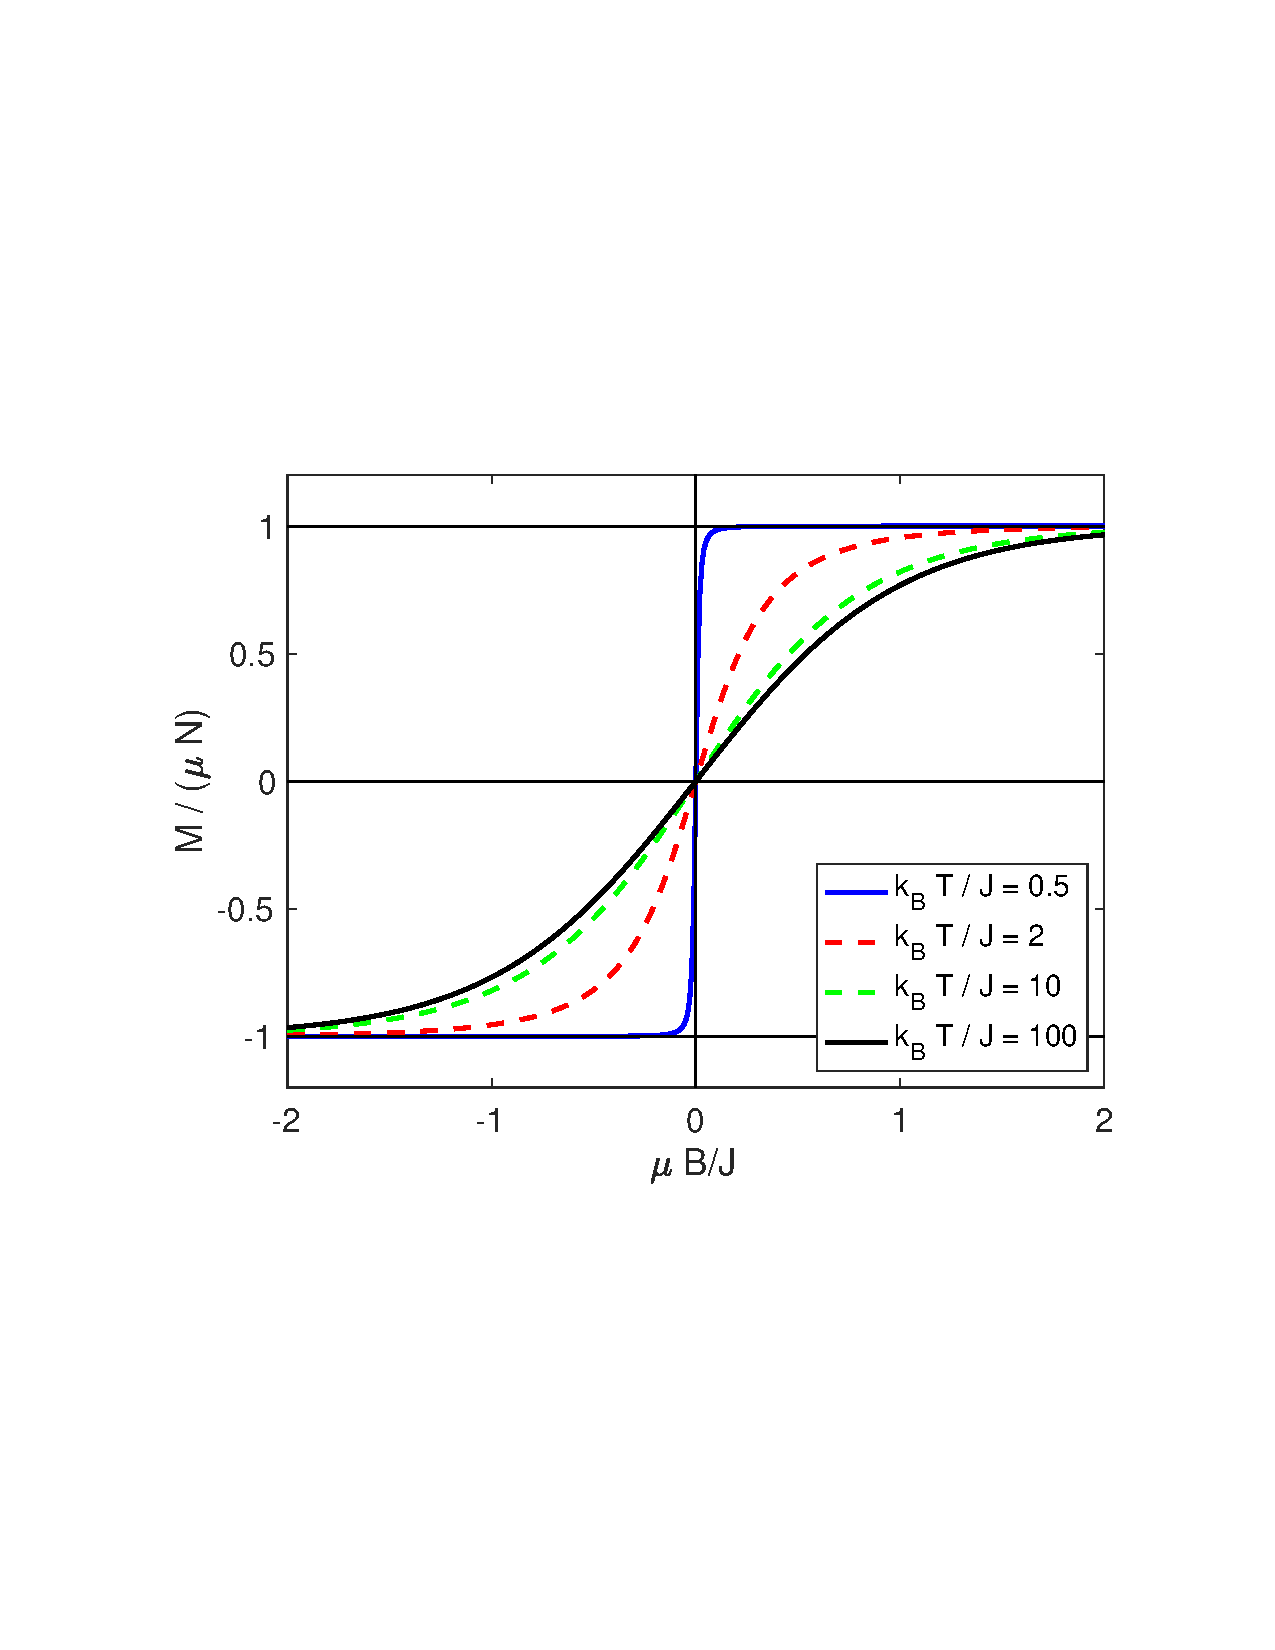
\includegraphics[width=10cm]{ising}
  \caption{Magnetization curve of the 1d Ising model.}
\end{figure}

We can see from the comparison with the result for the paramagnet that the amount of magnetization increases everywhere due to the influence of the interaction. For low temperatures, the magnetization abruptly enters the fully polarized state.

\section{Mean field approximation for any dimension}

(See {\em Ising Model for Magnetism (Springer)})

We will study the concept of the mean-field approximation in terms of the Ising model. 
We start out from  the Ising model expressed as
%
\begin{align*}
H &= - J \sum_{\langle ij\rangle} S_{i}S_{j} - 
B \cdot \hat M
\end{align*}
%
We recall that the Ising model describes spin-$1/2$ objects. 
The total magnetisation $\vv M$ is related to the spins
via 
%
\begin{align*}
\hat  M &=  \mu \sum_{i}
S_{i}\;.
\end{align*}
%
Now the Ising model takes only the component along the quantization axis into account and $S_{i}^{z}$ takes the values $\frac{\hbar}{2} \sigma_{i}$, with 
	$\sigma_{i}\in \{-1,+1\}$. 
%
As before, we introduce the  variable
%
\begin{align*}
h &= \mu  B\;.
\end{align*}
%
and obtain
\begin{align*}
H &= -J \sum_{\langle ij\rangle} S_{i}S_{j} - 
h \sum_{i} S_{i}
\end{align*}
Which is precisely the Hamiltonian of the Ising model. The mean field approximation is defined for any two dynamical variables $A$ and $B$
by
%
\begin{align*}
A B &\approx \langle A  \rangle B + A \langle B \rangle
-\langle A \rangle\langle B  \rangle\;.
\end{align*}
%
In our case, assuming translational invariance, we have
\begin{align*}
S_{i} S_{j}&\approx \langle S \rangle S_{j} + S_{i} \langle S \rangle
-\langle S \rangle^{2}\;.
\end{align*}
This leads to  the mean-field Hamilton function
%
\begin{align*}
H_\text{MFA} &= - J  \sum_{\langle ij\rangle}  \langle S \rangle S_{i}
- J  \sum_{\langle ij\rangle}  \langle S \rangle S_{j}
+J \sum_{\langle ij\rangle}  \langle S \rangle^{2}
  - h
\sum_{i} S_{i} \\
&= - 2J    \langle S \rangle \sum_{\langle ij\rangle} S_{i}
+J \sum_{\langle ij\rangle}  \langle S \rangle^{2}
  - h \sum_{i} S_{i} \\
\end{align*}
%
Since we have used the convention that the sum over nearest neighbours avoids
double counting, each site $i$ has $z/2$ nearest neighbours, where for simple cubic lattices $z=2d$ is defined as the total number of nearest neighbours.
Hence:
%
\begin{align*} %TODO: Added factor 1/2 here, is it correct?
H_\text{MFA} 
&= - J z  \langle S \rangle \sum_{i}  S_{i}
+ \frac{J N z}{2}  \langle S \rangle^{2}
  - h
\sum_{i} S_{i} \;.
\end{align*}
%
%
This can also be written as
\begin{align}\label{eq:ising:H:mfa}
H_\text{MFA} &=
  - h '\sum_{i} S_{i}
+ \frac{J N z}{2}  \langle S \rangle^{2}
 \\
\text{with }\qquad h' &= h + Jz \langle S \rangle\;.
\end{align}
The canonical partition function is then given by
%
\begin{align}\label{eq:ising:mfa:aux1}
Z(T,N,B) &= e^{-\frac{ \beta N J z}{2}\langle S \rangle^{2}} \sum_{\{S_{i}\}} e^{\beta h'\sum_{i}S_{i}}\;,
\end{align}
%
The partition function can easily be computed
%
\begin{align}\label{eq:}
Z(T,N,B) &= e^{-\frac{\beta N J z}{2} \langle S \rangle^{2}}\prod_{i} \sum_{S_{i}=\pm 1} e^{h' S_{i}} \nonumber\\
&= \bigg(  e^{\frac{-\beta J z}{2} \langle S \rangle^{2}}2 \cosh(\beta h') \bigg)^{N}\\
\ln\big( Z(T,N,B)  \big)
&= N \bigg( -\frac{\beta J z}{2} \langle S \rangle^{2} 
+\ln(2) 
+\ln\big( \cosh(\beta h')   \big) 
\bigg)
\label{eq:Z:Ising:MFA}
\end{align}
%
\subsection{Magnetization}
Next we compute the mean total spin ${\cal S}:=\sum_{i}S$
%
\begin{align*}
\avg{\cal S}
&=\frac{1}{Z}\sum_{\{S_{i}\}} 
\left\{ 
{\cal S} e^{-\frac{\beta N J z}{2}\langle S \rangle^{2}} e^{\beta h' {\cal S}}
\right\}
= \frac{k_{B}T}{Z} \frac{\partial }{\partial h'} Z\;.
\end{align*}
%
Hence
%
\begin{align}\label{eq:}
\avg{\cal S} &=k_{B}T\frac{\partial \ln(Z)}{\partial h'}
= N \tanh(\beta h')\;.
\end{align}
We introduce as $m$ the magnetization per site, divided by $\mu$
%
\begin{align}
m &= \frac{M}{\mu N} = \frac{1}{N}\langle\sum_{i}S_{i}  \rangle = \langle S \rangle\;.
\end{align}
%
%
and obtain the equation of state by using $h' = h + J z \langle S \rangle $ and dividing by $N$:
\tboxitp{Magnetization}{of the Ising model}{
%
\begin{align}\label{eq:eos:ising}
m &= \tanh\bigg( \beta \big(J z m + h\big)\bigg)\;.
\end{align}
%
}
We are particularly interested in the spontaneous magnetization, i.e. the magnetization for
$B\to 0 \Rightarrow h\to 0$. So we seek the solution of
%
\begin{align}\label{eq:magnetization:mfa}
m &= \tanh\big( \beta J z m\big)\;.
\end{align}
%
We introduce an auxiliary  temperature $T^{*}$, defined by
%
\begin{align}\label{eq:}
k_{B}T^{*} &= J z\;.
\end{align}
%
The condition for the spontaneous magnetization can therefore be expressed in a form and independent of the dimension
%
\begin{align}\label{eq:ising:mfa:mag}
m &=\tanh\big( \frac{T^{*}}{T} m \big)
\end{align}
%
or rather with $x = \frac{T^{*}}{T}m$
\begin{align}\label{eq:magnetization:mf}
x &= \frac{T^{*}}{T} \tanh\big( x \big)\;.
\end{align}
The function $\tanh(x)$ starts at $x=0$ with the value $0$ and slope 1, then it increases monotonically with  decreasing slope and approaches $1$ for $x\to \infty$.  
\eq{eq:magnetization:mf} has always the trivial solution $x=0 \Leftrightarrow  M=0$. For the non-trivial solution,
we need $\frac{T^{}*}{T}>1$, or rather $T<T^{*}$. According to the behaviour of $\tanh(x)$, for $\frac{T^{}*}{T}> 1$ there is precisely one non-trivial solution.
So we see that $T^{*}$ is indeed the critical/ Curie temperature, i.e
%
\begin{align}\label{eq:}
k_{B} T_{C}&=J z\;.
\end{align}
%

In 2D, we have $(\beta_{c} J)=.25$, as compared to the exact value $\beta_{c}J=0.4407$.
This not so bad, however, for 1D the mean-field result predicts a phase-transition at $(\beta_{c} J)=.5$, while the exact result is $\infty$.

In figure \ref{fig:M:mfa:ising}, the magnetization, obtained from \eq{eq:magnetization:mfa}, is depicted as function of $T$. Interestingly, the curve is independent of the spatial dimension.
The latter only enters in the value of $T_{c}$
\begin{figure}[t]
\begin{center}
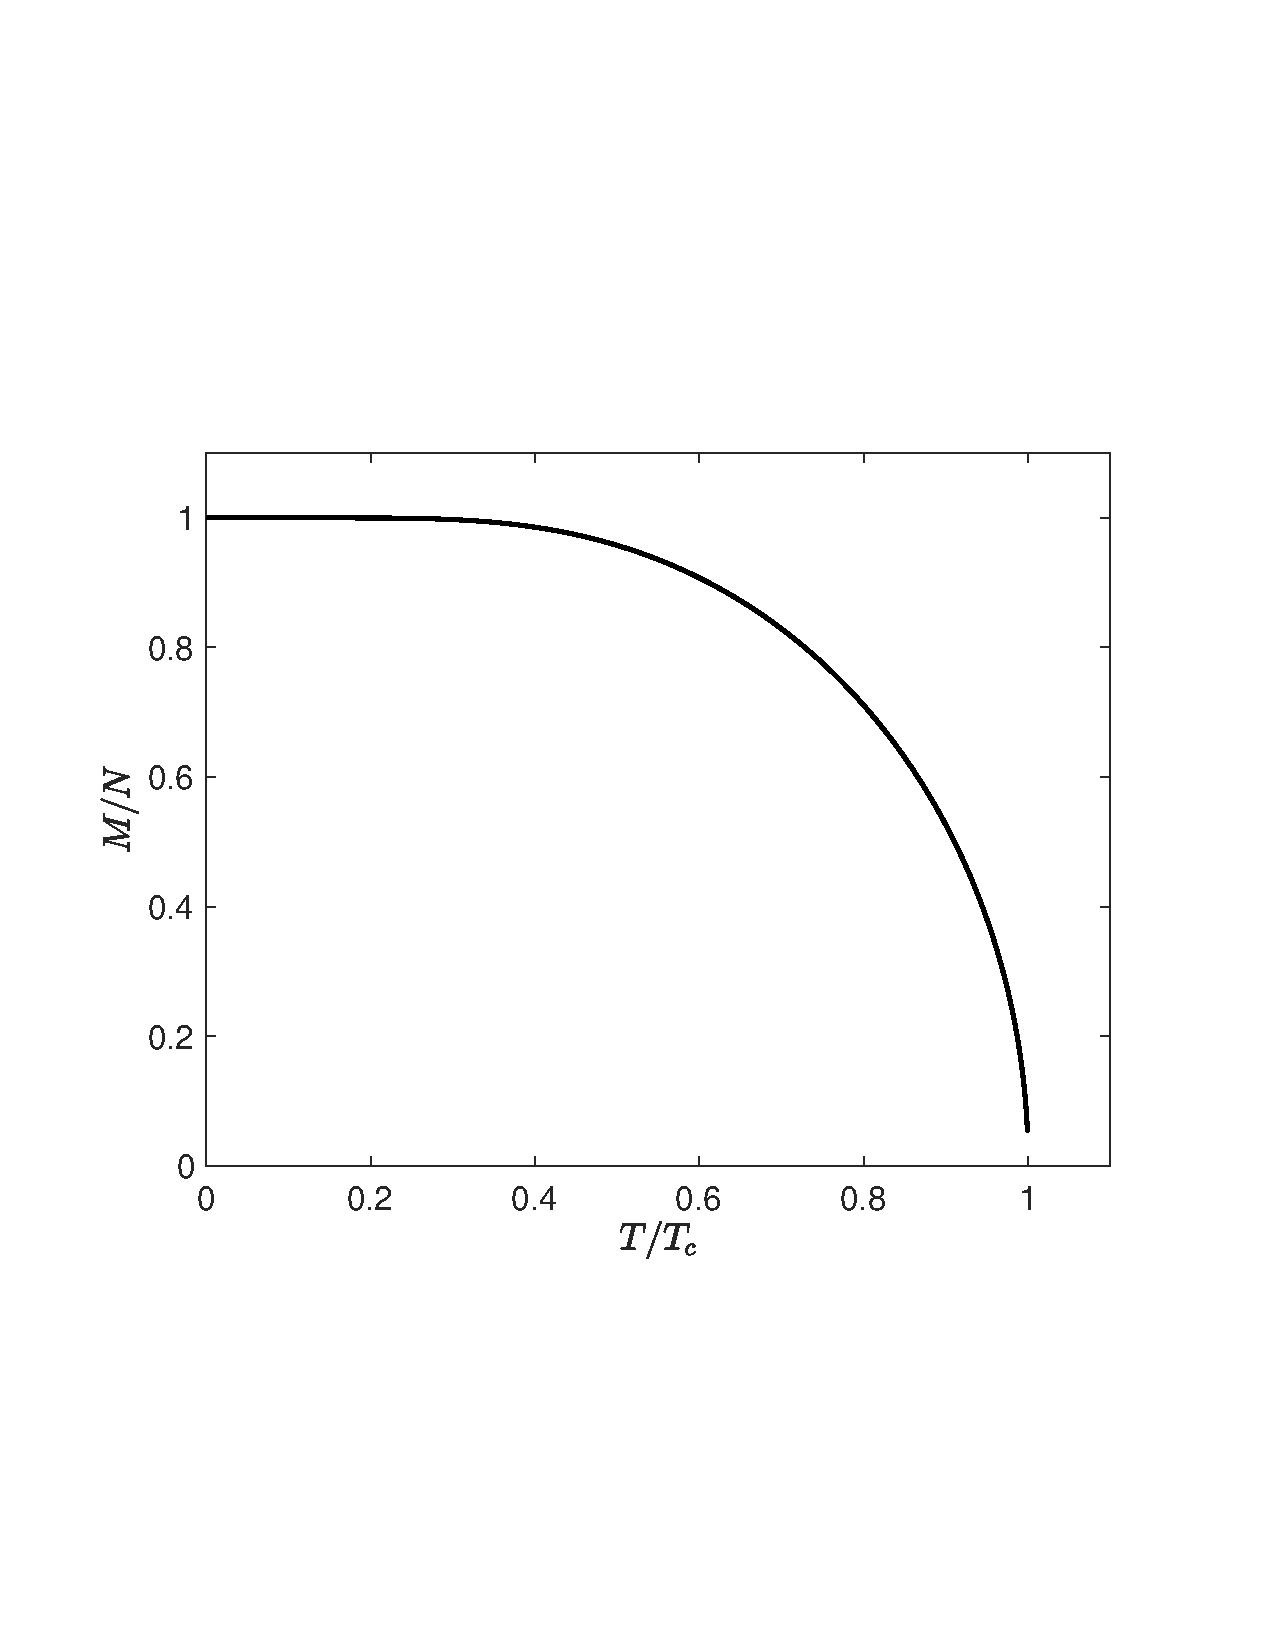
\includegraphics[width=7.5cm]{M_mfa_ising}
\caption{\it Mean-field result for the Magnetization for arbitrary spatial dimension $d$\label{fig:M:mfa:ising}}
\end{center}
\end{figure}

\subsubsection{Critical exponent}
For temperatures $T$ slightly below $T_{c}$, the magnetization is very small and we can use the Taylor expansion with $\tau = T/T_{C}$
\begin{align*}
m &= \tanh\big( \frac{m}{\tau} \big)= \bigg( \frac{m}{\tau} -\frac{(m/\tau)^{3}}{3} \bigg)
= \frac{m}{\tau}\bigg( 1- \frac{(m/\tau)^{2}}{3}\bigg)\\
\tau  &= 1 - \frac{(m/\tau)^{2}}{3}\\
\bigg(\frac{m}{\tau}\bigg)^{2} &= 3 \bigg( 1-\tau\bigg)\;.
\end{align*}

Up to this order we have for $T<T_{C}$
%
\begin{align}\label{eq:ising:mfa:m:Taylor}
m&= 3\tau \sqrt{1- \tau} \propto \varepsilon^{\frac{1}{2}}\\
\varepsilon &:= \frac{T_{C}-T}{T_{C}}
\end{align}
%
The  critical exponent is therefore $\beta=1/2$. 


\subsection{Magnetic susceptibility} %TODO: left out T=0?

Starting from the definition of the susceptibility via
%
\begin{align*}
\chi &= \frac{\partial M}{\partial B}\bigg|_{T,h=0}
\end{align*}
%
we obtain with $M=m N\mu$ and $B=h/\mu$ the relation 
%
\begin{align*}
\chi &= \left[ \frac{\partial M}{\partial m} \frac{\partial h}{\partial B} \frac{\partial m}{\partial h}  \right]_{T,h=0} = \mu^{2} N\pder{m}{h}{T,h=0}
\end{align*}
We start out from 
%
\begin{align*}
m &= \tanh\big(\beta h  +  \frac{T_{C}}{T} m\big)
\end{align*}
%
The derivative w.r.t. $h$ is
%
\begin{align*}
\xi=\pder{m}{h}{T, h=0} &=
\frac{\beta + \frac{T_{C}}{T} \xi}{\cosh^{2}\big( \beta h  +  \frac{T_{C}}{T} m \big)}\bigg|_{h=0}=
\frac{\beta + \frac{T_{C}}{T} \xi}{\cosh^{2}\big(\frac{T_{C}}{T} m \big)}\\
\xi \cosh^{2}\left(\frac{T_{C}}{T} m \right) &= \beta+ \frac{T_{C}}{T} \xi \\
\xi\bigg( \cosh^{2}\left(\frac{T_{C}}{T} m \right) - \frac{T_{C}}{T} \bigg) &= \beta\;.
\end{align*}
%
Close to $T_{C}$ the magnetisation is very small and we can Taylor expand the magnetisation
resulting in
%
\begin{align*}
\xi &= \frac{\beta}{ \cosh^{2}\big(\frac{T_{C}}{T} m \big) - \frac{T_{C}}{T} }\\
 &= \frac{\beta}{ 1 - \frac{T_{C}}{T} + \big( \frac{T_{C}}{T} m \big)^{2}}\\
 &= \frac{1}{k_{B}}\;\frac{1}{ T - T_{C}+  T_{C} \frac{T_{C}}{T} m^{2} }\;.
\end{align*}
%
We can replace $T$ by $T_{C}$ in the last term in the denominator, as it already contains $O(m^{2})$
%
\begin{align*}
\xi &= \frac{1}{k_{B}}\;\frac{1}{ T - T_{C}+  T_{C}  m^{2} }\;.
\end{align*}
%
{\bf For $T\searrow T_{C}$} the magnetisation is zero and we have 
\begin{align*}
\xi &= \frac{1}{k_{B} T_{C}} \;\big(\varepsilon\big)^{-1}
\end{align*}
with $\varepsilon=(T-T_{C})/T_{C}$.

\noindent
{\bf For $T\nearrow T_{C}$}  
we use  \eq{eq:ising:mfa:m:Taylor} for $m$ and obtain 
%
\begin{align*}
m^{2} &= 3 \tau^{2}\big( 1-\tau \big) = \frac{3}{T_{C}} \big( T_{C}-T \big) + {\cal O}(\Delta T/T_{C})^{2}
\end{align*}
%
and have
%
\begin{align*}
\xi &= \frac{1}{k_{B}}\;\frac{1}{ T - T_{C}+ 3  \big( T_{C}-T \big) }
= \frac{1}{2 k_{B}T_{C}}\abs{\varepsilon}^{-1}
\end{align*}
According to the definition of the critical exponent of the susceptibility 
%
\begin{align*}
\chi \simeq A_{\pm } \abs{\varepsilon}^{-\gamma_{\pm}}
\end{align*}
%
we have $A_{+}= 2 A_{-}$ and $\gamma_{+}=\gamma_{-}=1$.
%
\subsection{Free energy}
Next we compute the free energy based \eq{eq:Z:Ising:MFA}
%
\begin{align*}
f:=\frac{F}{k_{B} N} &=-\frac{k_{B}T}{k_{B} N} \ln(Z)\\
&=-T \bigg( -\frac{\beta J z}{2} \langle S \rangle^{2} 
+\ln(2) 
+\ln\big( \cosh(\beta h')   \big) 
\bigg)\\
%&=- T 
%\bigg[
%\frac{- \beta J z}{2} m^{2}  +
%\ln\big(2\cosh(\beta h + \frac{Jz}{k_{B}T}m)  \big)\bigg]\\
&=
\frac{J z}{2 k_{B}} m^{2}  - T
\ln\big(2\big)  - T\ln\big( \cosh(\beta h + \frac{J z}{k_{B}T} m)\big)\;.
\end{align*}
%
The natural variables are  $T$, $N$, and $h$.
However, we will see that the magnetization $m$ is more suitable than $h$ and we will
introduce a corresponding Legendre transformation later.

We have seen before that $k_{B} T_{C} = J z$ so we can 
express the free energy as
%
\begin{align*}
\frac{F}{N k_{B}} &= \frac{1}{2} T_{c} m^{2}
-  T\ln\big(2\big) - T\ln{ \cosh(\beta h + \frac{T_{c}}{T} m)  }\;.
\end{align*}
%
Along with
%
\begin{align*}
\cosh(x) &= \big(1-\tanh^{2}(x)\big)^{-1/2} 
\end{align*}
and the self consistency \eq{eq:ising:mfa:mag}
%
\begin{align}\label{eq:magnetization}
m &= \tanh\big( \beta h + \frac{T_{C}}{T} m \big)
\end{align}
%
we can express the free energy as
%
\begin{align}\label{eq:isingh:mfa:F}
\frac{F}{N k_{B}} &= \frac{T_{c} m^{2}}{2} 
-  T\ln\big(2\big)  + \frac{T}{2} \ln\big(1-m^{2}\big)\;.
\end{align}
%

Next we compute the Helmholtz free energy, by the following Legendre transform, where we introducing $M$ as  natural variable instead of $h$:
%
\begin{align}
A(T,M) &= F(T,h) + Mh\;.
\end{align}
%
Then the total differential reads
%
\begin{align*}
dA  &= dF(T,h) + h dM +M dh\\
&= -S dT - M dh + h dM +M dh  \\
&= -S dT + h dM\;.
\end{align*}
%
\blue{exercise: proof  $\frac{\partial F}{\partial h}= - M $ by using \eq{eq:isingh:mfa:F} and \eq{eq:magnetization}.}
Hence 
%
\begin{align}\label{eq:MFA:dA:dM}
\pder{A}{M}{T} &= h\\
\pder{A}{T}{M} &= -S\;.\label{eq:MFA:S}
\end{align}
%
%
If we want to have spontaneous magnetisation,  i.e. a finite magnetisation $M$
without external field, then according to \eq{eq:MFA:dA:dM} we are looking for 
a finite value of the magnetization $M$ for which
%
\begin{align}\label{eq:MFA:dA:dM:zero}
\pder{A(M,T)}{M}{T} &= 0\;.
\end{align}
%
Before we can exploit this equation, we need to express $h$ in  terms of $M$ (or rather $m$).
To this end we invert 
%
\begin{align*}
m &= \tanh\bigg(\beta h + \frac{T_{C}}{T} m\bigg)
\end{align*}
%
leading to
%
\begin{align*}
\beta h + \frac{T_{C}}{T} m  &= \tanh^{-1}\big(m\big)\;.
\end{align*}
%
Along with 
\begin{align*}
\text{tanh}^{-1}\big(b\big)=\frac{1}{2}\ln\bigg( \frac{1+b}{1-b} \bigg)
\end{align*}
we obtain
%
\begin{align*}
\beta h +\frac{T_{c}}{T}m &= 
\frac{1}{2}\ln\bigg( \frac{1+m}{1-m} \bigg)\\
h &= \frac{k_{B}T}{2}\ln\bigg( \frac{1+m}{1-m} \bigg)
-k_{B}T_{c} m
\end{align*}
%
Then we obtain for the Helmholtz free energy of \eq{eq:isingh:mfa:F}
%
\begin{align*}
\frac{A}{N k_{B}} &= \frac{T_{C} m^{2}}{2} -T\ln(2) +\frac{T}{2} \ln\big( 1-m^{2} \big) + \frac{mh}{k_{B}}\\
 &=\frac{1}{2} T_{c} m^{2}
-  T\ln(2) + \frac{T}{2}\ln\big(1-m^{2} \big)
+ \frac{m }{k_{B}}
\bigg( \frac{k_{B}T}{2} \ln\bigg( \frac{1+m}{1-m} \bigg)
- k_{B}T_{c}m
\bigg)\\
 &=\frac{1}{2} T_{c} m^{2}
-  T\ln(2) + \frac{T}{2}\ln\big(1-m^{2} \big)
+
\frac{m T}{2}\ln\bigg( \frac{1+m}{1-m} \bigg)
- T_{c} m^{2}
\;.
\end{align*}
%
or rather
%
\begin{align}\label{eq:sing:mfa:S}
\frac{A}{N k_{B} T_{c}}= \frac{A}{N J z}&=-\frac{1}{2} m^{2}
-\tau\ln(2) + \frac{\tau}{2}\bigg[\ln\big((1-m)(1+m) \big)
+ m \ln\bigg( \frac{1+m}{1-m} \bigg)\bigg]\notag\\
&=-\frac{1}{2} m^{2}
-\tau\ln(2) + \frac{\tau}{2}
\bigg( 
\big(1+m\big) \ln\big(1+m \big) + \big(1-m\big) \ln\big(1-m \big)
 \bigg)\;,
\end{align}
%
%
with $\tau =T/T_{c}$.
%
\begin{figure}[h]
\begin{center}
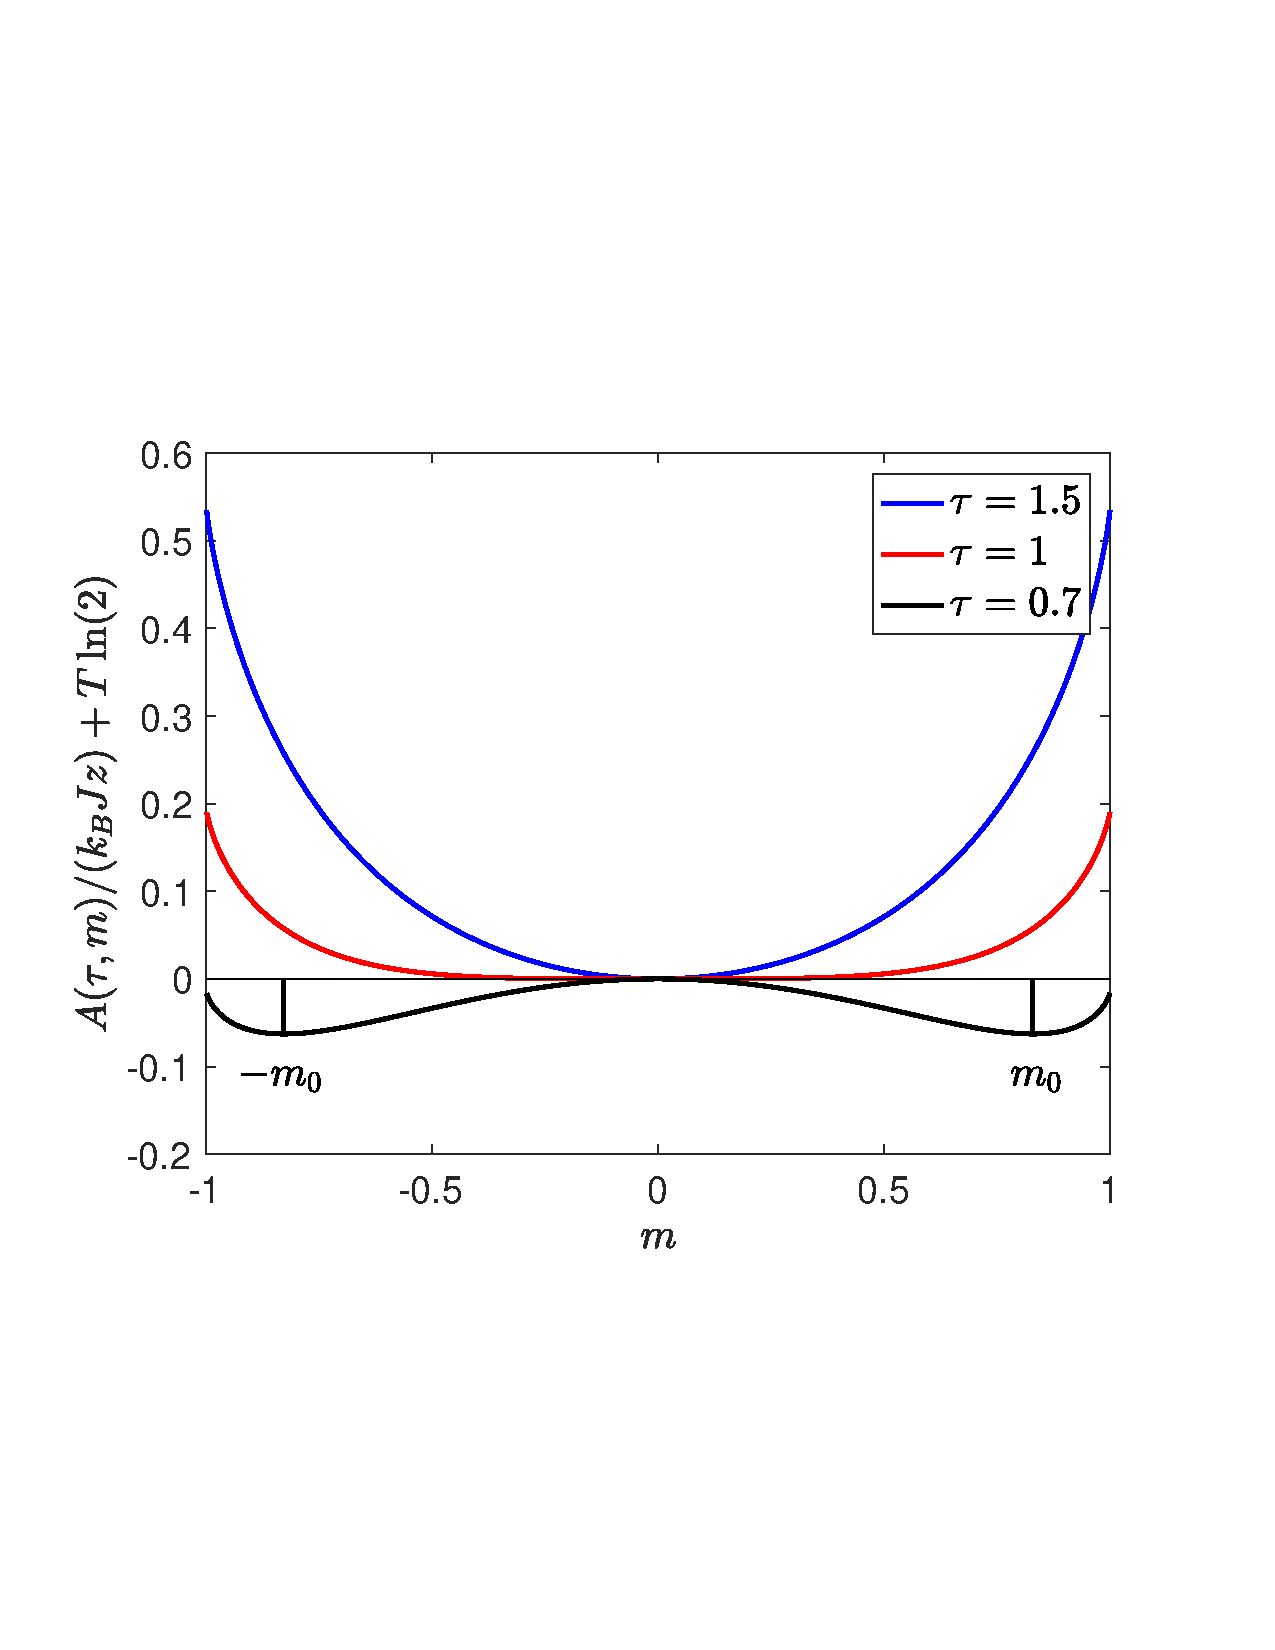
\includegraphics[width=7.5cm]{freeEnergyHemlholz}
\caption{{\it Helmholtz free energy for the Ising model in mean-field approximation versus order parameter without external field.}\label{fig:freeEnergyHemlholz}}
\end{center}
\end{figure}
%
According to \eq{eq:MFA:dA:dM:zero} the magnetization is given by the points where the slope as function of $m$ vanishes (see figure \ref{fig:freeEnergyHemlholz}).

\newpage 

\subsection{Entropy}


\begin{figure}[t]
\begin{center}
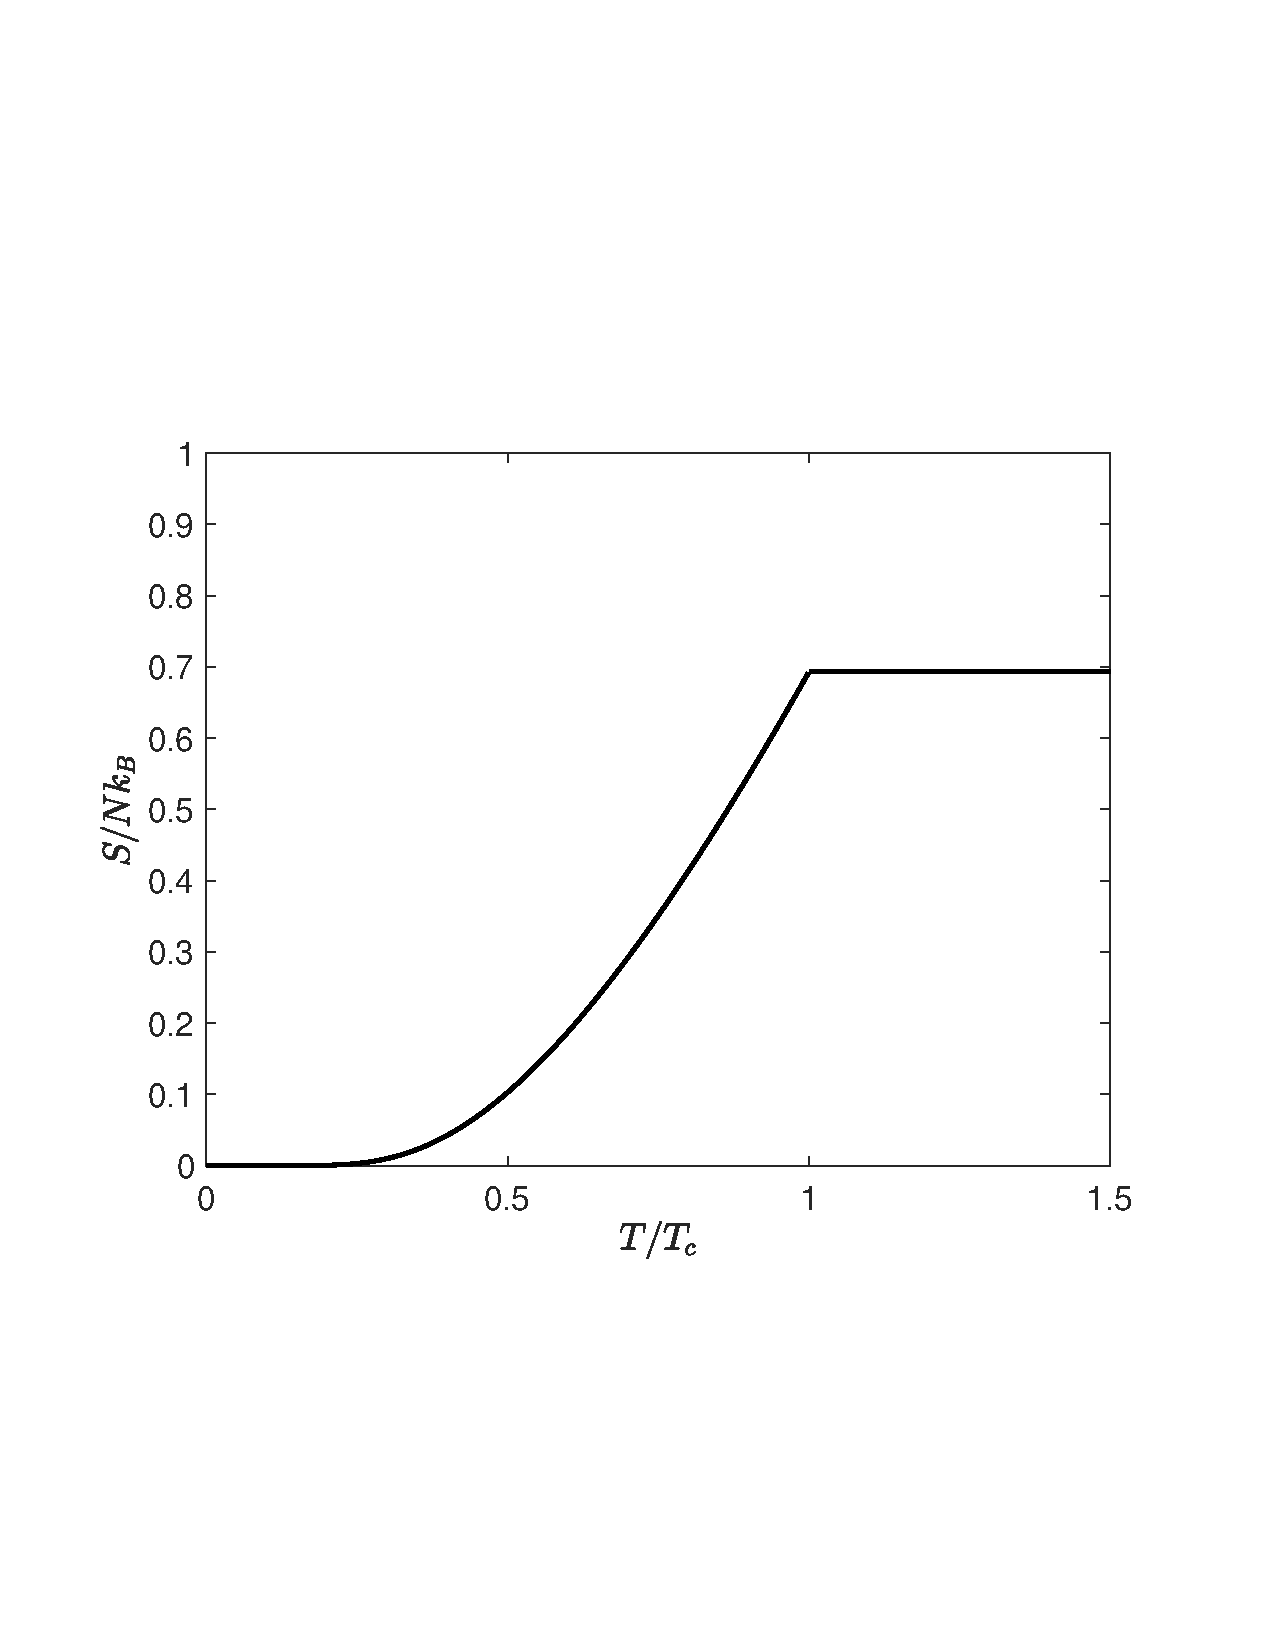
\includegraphics[width=7.5cm]{S_mfa_ising}
\caption{{\it Entropy of the Ising model in MFA.}}
\end{center}
\end{figure}

According to \eq{eq:MFA:S} , which was
%
\begin{align*}
S &= -\pder{A}{T}{M} 
\end{align*}
%
along with \eq{eq:sing:mfa:S}
the entropy is
%
\begin{align*}
-\frac{S}{N k_{B}T_{C}} &=
\frac{\partial }{\partial \tau} \bigg( 
-\frac{1}{2} m^{2}
-\tau\ln(2) + \frac{\tau}{2}
\bigg( 
\big(1+m\big) \ln\big(1+m \big) + \big(1-m\big) \ln\big(1-m \big)
 \bigg)
\bigg)\bigg|_{m} \frac{d \tau }{dT}\nonumber\;.
\end{align*}
%
Hence
%
\tboxitp{Entropy of the Ising model}{in MFA for zero field}{
\begin{align}
\label{eq:ising:mfa:entropy}
\frac{S}{N k_{B}}
&=
\ln(2) - \frac{1}{2}
\bigg(\big( 1+m \big)\ln\big(1+m\big) +
\big(1-m\big) \ln\big(1-m\big) \bigg)\;. 
\end{align}}
%

It has the correct limiting behaviour: For $T\to0$, i.e. $m\to 1$ we obtain
%
\begin{align*}
\frac{S}{N k_{B}} &= \ln(2) -\frac{1}{2}\bigg( 2\bigg( \ln(2) + 0 \bigg) \bigg) = 0\;,
\end{align*}
%
and for $T\to\infty$, i.e. $m\to 0$ the entropy becomes
%
\begin{align*}
\frac{S}{N k_{B}} &= \ln(2) -\frac{1}{2}\bigg( 
\ln(1) + \ln(1)  \bigg) = \ln(2)\;.
\end{align*}
%
Recall that
%
\begin{align*}
S &= k_{B} \ln( \text{number of micro states})\;.
\end{align*}
%
For $T\to \infty$ all states can be reach with the same probability. Hence the number of micro states is $2^{N}$ and
%
\begin{align*}
S &= N k_{B} \ln( 2)\;,
\end{align*}
%
in agreement with the above result.

For the entire $T$ dependence of $S$ we have to insert the self-consistent solution for $m(T)$ in \eq{eq:ising:mfa:mag}.
%
  \subsection{Internal Energy}
The internal energy is defined as the expectation value of the hamiltonian.
Using the mean field expression of \eq{eq:ising:H:mfa} we have
%
\begin{align*}
U &=
%\langle H \rangle = -h' \sum_{i} \langle S_{i} \rangle + \frac{J N z}{2} m^{2}=
 N\big(-h'  m + \frac{J  z}{2} m^{2}\big)
\intertext{with $ h' =J z m + h$ we obtain:} 
%&= -J z m^{2} - h m  + \frac{J  z}{2} m^{2}\\
\frac{U}{NJ }&= -\frac{h m }{J} - z m^{2} + \frac{z}{2}m^{2}\\
&= - \frac{z}{2} m^{2} - \frac{h m }{J}\;.
\end{align*}
%
For zero external field it simplifies to (we also use $z=2d$)
%
\tboxitp{Internal energy of the Ising model}{in MFA for zero field}{
\begin{align}
\frac{U}{NJ }&= - d\; m^{2} \;.
\end{align}}
%


\subsection{Specific heat}
For the specific heat we need
%
\begin{align*}
C_{h=0} &= \pder{U}{T}{h=0} = - d N J   \;\frac{d\; m^{2} }{d T} \\
\frac{C_{h=0}}{N J} &= -d\;   \;\frac{d }{d T}  m^{2}\;.
\end{align*}
%
Above $T_{C}$ the magnetization is zero and hence $C = 0$.
Slightly below $T_{C}$ we can replace $m$ by \eq{eq:ising:mfa:m:Taylor}, which gives

\begin{align*}
\frac{C_{h=0}}{N J} &= -d   \;\frac{d   }{d T}  3 \tau^{2}\big( 1-\tau \big)\\
&=- \frac{3d}{T_{C}^{3}}   \;\frac{d   }{d T}   \big( T^{2} T_{C}- T^{3} \big)\\
&=- \frac{3d}{T_{C}^{3}}   \;T\; \big( 2  T_{C}- 3 T \big)\;.
\end{align*}
Hence, approaching $T_{C}$ from below we obtain
%
\begin{align}\label{spec:heat:MFA}
\frac{C(T_{C})_{h=0}}{N J}
&= \frac{3d}{T_{C}} =  \frac{3d k_{B}}{J z} =\frac{3d k_{B}}{J 2d}\\
\frac{C(T_{C})_{h=0}}{N} &= \frac{3k_{B}}{2}\;.
\end{align}
%
Therefore, in MFA, the specific heat has no power-law behaviour close at $T_{C}$, but rather a 
discontinuity from $\frac{3}{2}k_{B}$ below $T_{C}$ to 0 above $T_{C}$.
For the entire $T$-dependence below $T_{C}$ we continue with
%
\begin{align}
\frac{C_{h=0}}{N J} &= - 2 d\;   m\;\frac{d m}{d T} \;.
\end{align}
%
First we consider
%
\begin{align*}
\xi :=\;\frac{d m}{d T}  \;.
\end{align*}
%
Exploiting \eq{eq:magnetization} yields
\begin{align}
\xi &= \frac{d}{dT} \tanh\big( \beta h + \beta k_{B} T_{C} m \big)\bigg|_{h=0}\\
\xi &= \frac{(h +  k_{B} T_{C} m )\frac{ d \beta}{dT} + \beta k_{B}T_{C} \xi}{\cosh^{2}\big( \beta (h +  k_{B} T_{C} m )\big)}\bigg|_{h=0}\\
 &= \frac{-\frac{T_{c}}{T^{2}}  m + \frac{T_{C}}{T} \xi}{\cosh^{2}\big( \frac{T_{C}}{T} m \big)}\;.
\end{align}
%
Then
%
\begin{align*}
\xi \cosh^{2}\big( \frac{T_{C}}{T} m \big) 
 &= -\frac{T_{c}}{T^{2}}  m + \frac{T_{C}}{T} \xi\\
\xi \bigg(\cosh^{2}\big( \frac{T_{C}}{T} m \big) -\frac{T_{C}}{T}\bigg)
 &= -\frac{T_{C}}{T^{2}}  m \\
\xi &= -\frac{1}{T_{C}}\;
\frac{\frac{m}{\tau}}{ \tau \cosh^{2}\big( \frac{m}{\tau} \big) - 1 }
\end{align*}
%
That leads to
%
\begin{align*}
\frac{C_{h=0}}{N J} &= - z\;   m\;\xi\\
&=\frac{z}{T_{C}} 
\frac{\frac{m^{2}}{\tau}}{ \tau \cosh^{2}\big( \frac{m}{\tau} \big) - 1 }\\
&=\frac{z}{z J/k_{B}} 
\frac{\frac{m^{2}}{\tau}}{ \tau \cosh^{2}\big( \frac{m}{\tau} \big) - 1 }\;.
\end{align*}
%
Finally, we have 
%
\begin{align}\label{eq:}
\frac{C_{h=0}}{N} &=k_{B 	}
\frac{\big(\frac{m}{\tau}\big)^{2}}{ \cosh^{2}\big( \frac{m}{\tau} \big) - 1/\tau }\;.
\end{align}
%
%
Together with the self consistent equation for $m(T)$:
%
\begin{align*}
m(T) &= \tanh\bigg(\frac{T_{C}}{T} m(T)\bigg)\;,
\end{align*}
%
which have solved numerically before, we can plot the specific heat.
\begin{figure}[t]
\begin{center}
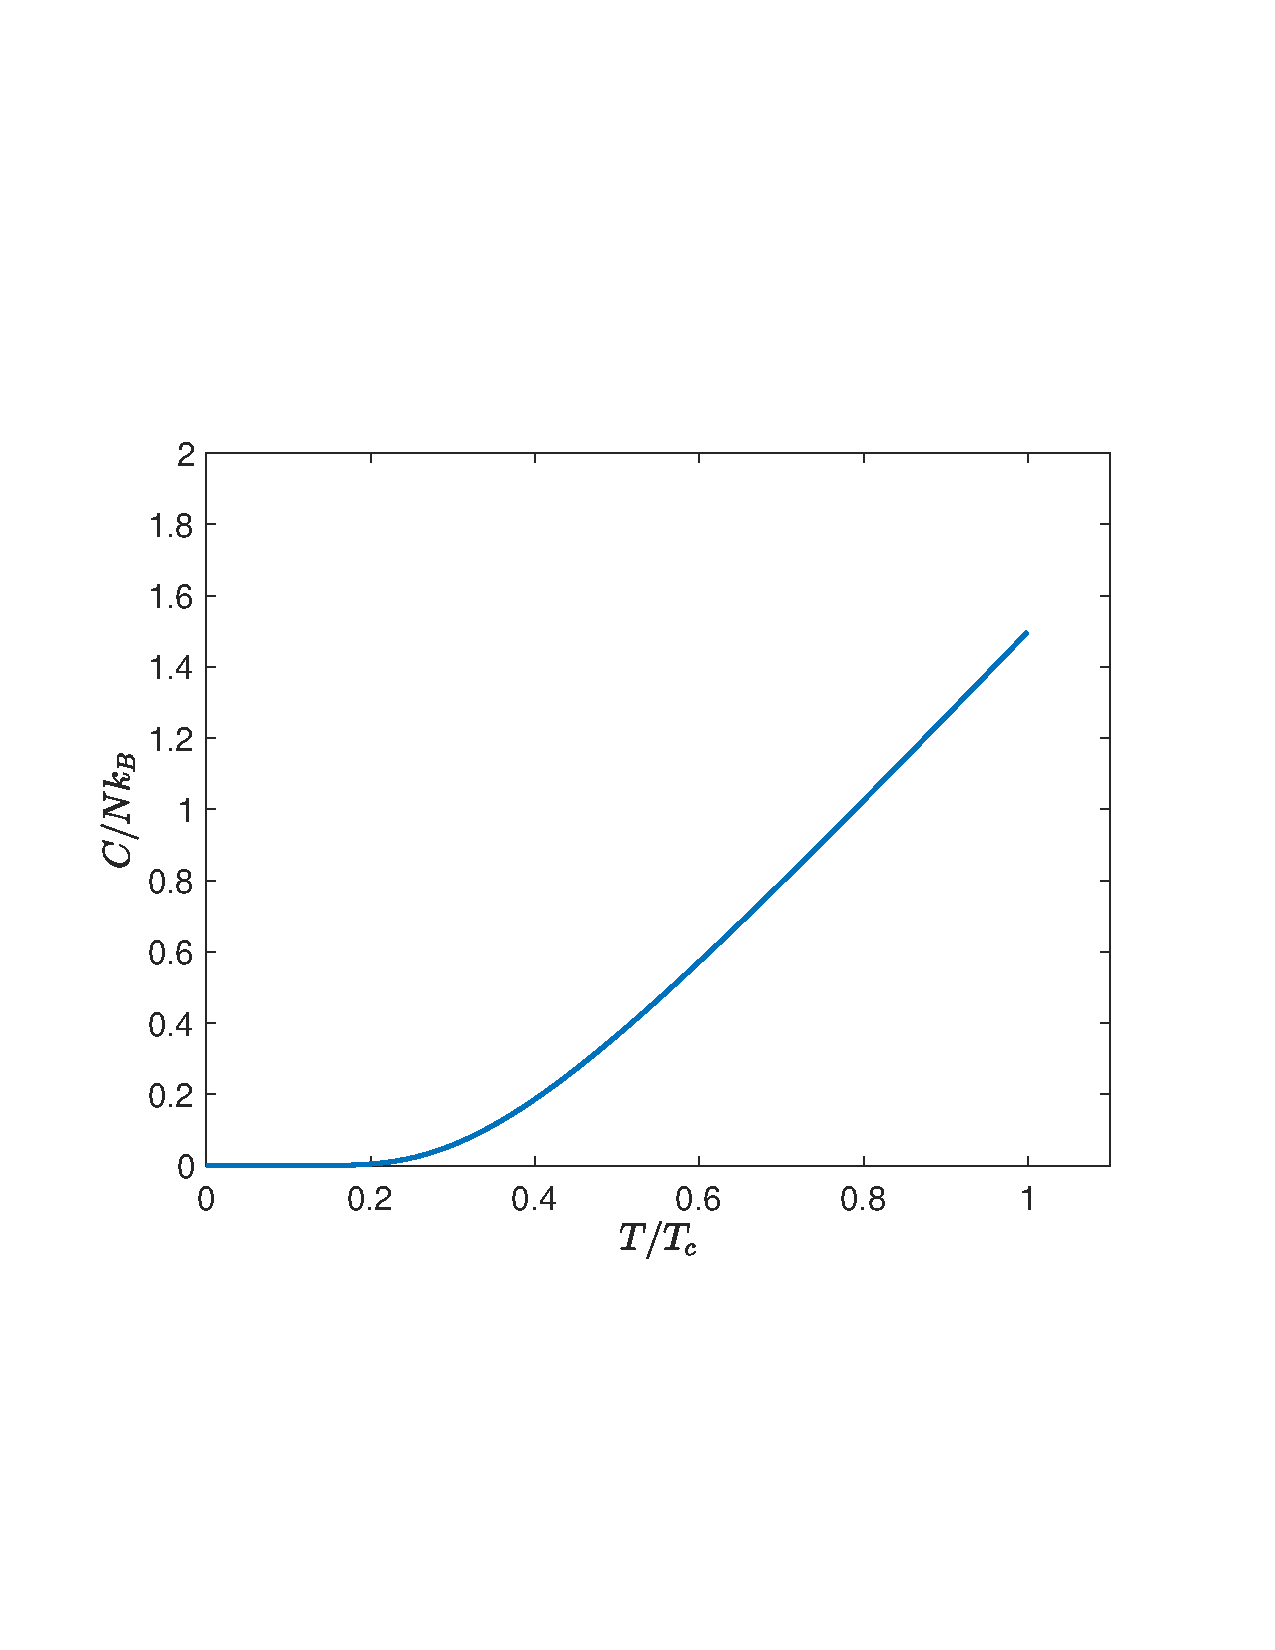
\includegraphics[width=7.5cm]{C_mfa_ising}
\caption{{\it Specific heat of the Ising model in MFA.}}
%TODO: Include also a plot of the internal energy in this
\end{center}
\end{figure}

We have seen in  'statistical physics I' 
%
\begin{align*}
C&= \frac{1}{k_{B} T^{2}} \avg{\big( \Delta H \big)^{2}}\;,
\end{align*}
%
i.e. $C$ is large when there are pronounced energy fluctuations,
which is the case in the vicinity of $T_{C}$.
In  MFA, above $T_{C}$ there are no fluctuations because
$H \propto m$ and therefore $U=0$ aboce $T_{C}$.
This is an artefact of MFA.


\section{Exact solution of the 2d Ising model}
\subsection{Transfermatrix approach}
We will first briefly explain how the Transfer matrix approach works in the 2d case.
To this end we will represent the hamiltonian of the 2d Ising model ($L_{x}\times L_{y}$)
by writing the two cartesian indices explicitly in the form
$S_{ij}$
%
%
\begin{align*}
-\beta H &= j \sum_{l=1}^{L_{y}} \sum_{i=1}^{L_{x}}	\qty( S_{i,l}S_{i+1,l} +S_{i,l}S_{i,l+1})
+ h \sum_{l} \sum_{i} S_{il}\;.
\end{align*}
%
Now we combine the spins of column $l$  (i.e. $S_{il}$) in a vector
%
\newcommand{\vS}[1]{{ \mathbf {\cal  S}^{(#1)}}}
\newcommand{\vSx}{{ \mathbf {\cal  S}}}
\newcommand{\vSp}{{ \mathbf {\cal  S}'}}
\begin{align*}
\vS{l} &= 
\begin{pmatrix}
S_{1,l}\\
S_{2,l}	\\
\ldots\\
S_{L_{x},l}
\end{pmatrix}\;,
\text{i.e. }(\vS{l})_{i} = S_{il}
\end{align*}
%
Then the hamiltonian can be written as
%
\begin{align}\label{eq:beta:H}
-\beta H &= \sum_{l}  A\big(\vS{l}, \vS{l+1}\big)\\
\intertext{with the definitions}
A(\vS{l},\vS{k}) &= \frac{1}{2}\bigg(\tilde A(\vS{l},\vS{k}) + \tilde A(\vS{k},\vS{l}) \bigg) \\
\tilde A(\vS{l},\vS{k}) &= 
j \sum_{i}  \bigg((\vS{l})_{i} (\vS{l})_{i+1}  +(\vS{l})_{i} (\vS{k})_{i}\bigg)
+ h \big(\sum_{i} \vS{l})_{i}\;.
\end{align}
%
$A$ is by construction a real symmetric matrix.
Inserting indices yields
%
\begin{align*}
\sum_{l} \tilde A(\vS{l},\vS{l+1}) &= 
 j \sum_{l,i}\big(  S_{i,l}S_{i+1,l} +S_{i,l}S_{i,l+1}\big)
+ h \sum_{i,l} S_{i,l} &&= - \beta H\\
\sum_{l} \tilde A(\vS{l+1},\vS{l}) &= 
 j \sum_{l,i}\big(  S_{i,l+1}S_{i+1,l+1} +S_{i,l+1}S_{i,l}\big)
+ h \sum_{i,l} S_{i,l+1} \\
(l+1 \to l'  \text{ plus pbc} \Rightarrow)\qquad 
&= j \sum_{l',i}\big(  S_{i,l'}S_{i+1,l'} +S_{i,l'}S_{i,l+1}\big)
+ h \sum_{i,l} S_{i,l'} &&= - \beta H\;.
\end{align*}
%
Hence \eq{eq:beta:H} is correct.
Then 
%
\begin{align*}
Z &= \sum_{\{S_{ij}\}} e^{\sum_{l=1}^{L} A(\vS{l},\vS{l+1}) }
 = \prod_{l=1}^{L} \sum_{\vS{l}}  e^{ A(\vS{l},\vS{l+1}) }\;.
\end{align*}
%
Now, we introduce the transfer matrix ${\cal T}$ with matrix elements
%
\begin{align*}
{\cal T}_{\vS{l},\vS{l'}} &= e^{A\big(\vS{l},\vS{l'}\big)}
\end{align*}
%
Then the partition function can be written as (remember that we use pbc)
%
\begin{align*}
Z &= \sum_{\vS{1}} \sum_{\vS{2}}\cdots  \sum_{\vS{L_{y}}}\prod_{l} {\cal T}_{\vS{l},\vS{l+1}}\\
&= \sum_{\vS{1}} \sum_{\vS{2}}\cdots  \sum_{\vS{L_{y}}} {\cal T}_{\vS{1},\vS{2}}{\cal T}_{\vS{2},\vS{3}}\cdots {\cal T}_{\vS{L_{y}-1},\vS{L_{y}}}
 {\cal T}_{\vS{L_{y}},\vS{1}}\\
&= \tr{{\cal T}^{L_{y}}} \\
&= \lambda_\text{max}^{L_{y}}\;.
\end{align*}
%
This is the straight-forward generalization of \eq{eq:transfer:1d}
and  is to be understood as follows: 
The sum over $\vS{l}$ runs over 
the $2^{L_{x}}$ configurations, which the vector $\vS{l}$ can assume. 
We introduce an index $I$ that enumerates these configurations and 
instead of summing over $\vS{l}$, we could sum over the index $I$ , that enumerates 
these configurations (the $I$-the configuration would be ${\cal S}_{I}$). Then we can define the transfer matrix alternatively by the matrix elements
\begin{align*}
{\cal T}_{I,I'} &= e^{A({\cal S}_{I}, {\cal S}_{I'})}
\end{align*}
%
and then we would have
%
\begin{align*}
Z &=  \sum_{I^{(1)}} \cdots  \sum_{I^{(L_{y})}} {\cal T}_{I^{(1)},I^{(2)}}
{\cal T}_{I^{(2)},I^{(3)}},\ldots,{\cal T}_{I^{(L_{y}-1)},I^{(L_{y})}}
{\cal T}_{I^{(L_{y})},I^{(1)}}\\
&= \tr{{\cal T}^{L_{y}}} \\
&= \lambda_\text{max}^{N}\;.
\end{align*}
%

%
As before, the dominant eigenvector ($\lambda_\text{max}$) predominates in the thermodynamic limit ($L_{y}\to \infty$). The eigenvalue problem
of the  ($2^{L_{x}}\times 2^{L_{x}}$)-dimensional transfer matrix for the 2d case, is much more complicated than  in the
1d case. It can be found in the book of K. Huang
({\em Kerson Huang, Statistical Mechanics, Wiley and Sons (1963)}).

\subsection{Graphical approach \blue{(Bachrlor thesis J. Pomper)}}
Here we will present instead the exact solution of the 2d Ising model based a graphical representation, however, without external field.
The  ideas go back to M. Lawrence Glasser, American Journal of Physics 38, 1033 (1970), and were
didactically improved by W. Noting: Qauntum Therory of Magnetism (Springer Verlag).

Starting point is the partition function
%

\begin{align}\label{eq:Ising:2d:Z}
Z &= \sum_{\{S_{i}\}} \prod_{\langle ij \rangle} e^{j S_{i}S_{j}}\;.
\end{align}
%
Next we expand the exponential in a Taylor series
%
\begin{align*}
 e^{j S_{i}S_{j}} 
&= \sum_{n=0}^{\infty}\frac{j^{n}}{n!} \big( S_{i}S_{j} \big)^{n}\\
&= \sum_{n=0}^{\infty}\frac{j^{2n}}{(2n)!} \underbrace{
\big( S_{i}S_{j} \big)^{2n}
}_{\color{blue} = 1}
+\sum_{n=0}^{\infty}\frac{j^{2n+1}}{(2n+1)!} \underbrace{
\big( S_{i}S_{j} \big)^{2n+1}
}_{\color{blue} = S_{i}S_{j}}\\
&= \cosh(j)\big(1 + \tanh(j) S_{i}S_{j}\big)
\end{align*}
%
Inserted in \eq{eq:Ising:2d:Z} results in
%
\begin{align*}
Z&= \cosh^{2N}(j) \;\sum_{\{S_{i}\}}\;\prod_{\langle ij \rangle} \big( 1+ t S_{i} S_{j}\big)\;,
\end{align*}
%
where  $t=\tanh(j)$. The power $2N$ arises as there are $2N$ terms in the product in \eq{eq:Ising:2d:Z}. For each factor we have the choice to use
the term $1$ or $t S_{i}S_{j}$. In total there are $2^{Nz}$ such terms, for which we still have to sum over all spin configurations. Graphically, we represent the terms $t S_{i}S_{j}$ as lines 
on a square lattice connecting site $i$ and $j$. Such a line can be considered as {\em edge of a a graph} and the sites that are connected by edges are 
denoted as  {\em vertices}. In graph theory the number of edges connected to a vertex is called {\em order of the vertex}. In the present context, it can only be
an integer $n\in\{0,1,2,3,4\}$.
Each edge, that reaches site (vertex)  $i$  carries a factor $S_{i}$. Therefore, we obtain a term $S_{i}^{n}$, where $n$ is the order of the vertex. $n\in\{0,1,2,3,4\}$. If the order is odd, the sum over $S_{i}$ vanishes, otherwise it gives $2$. 
Hence, only graphs where all vertices have an even order (either $0$, $2$ or $4$) are allowed. By now we have
\begin{align*}
Z&=2^{N}\; \cosh^{2N}(j) \;\sum_{G} t^{N_{e}(G)}\;,
\end{align*}
The sum runs over all possible graphs on a square lattice of given size, with periodic boundary conditions, with vertices of even order.
$N_{e}(G)$ is the total number of edges of the graph. The elements of the individual graphs need not to be connected.
In \fig{fig:graph:ising} two examples are given, one for an allowed and one for a forbidden 
graph.
%
\begin{figure}[t]
\subfigure[Allowed graph with $N_{e}(G)=20$.]{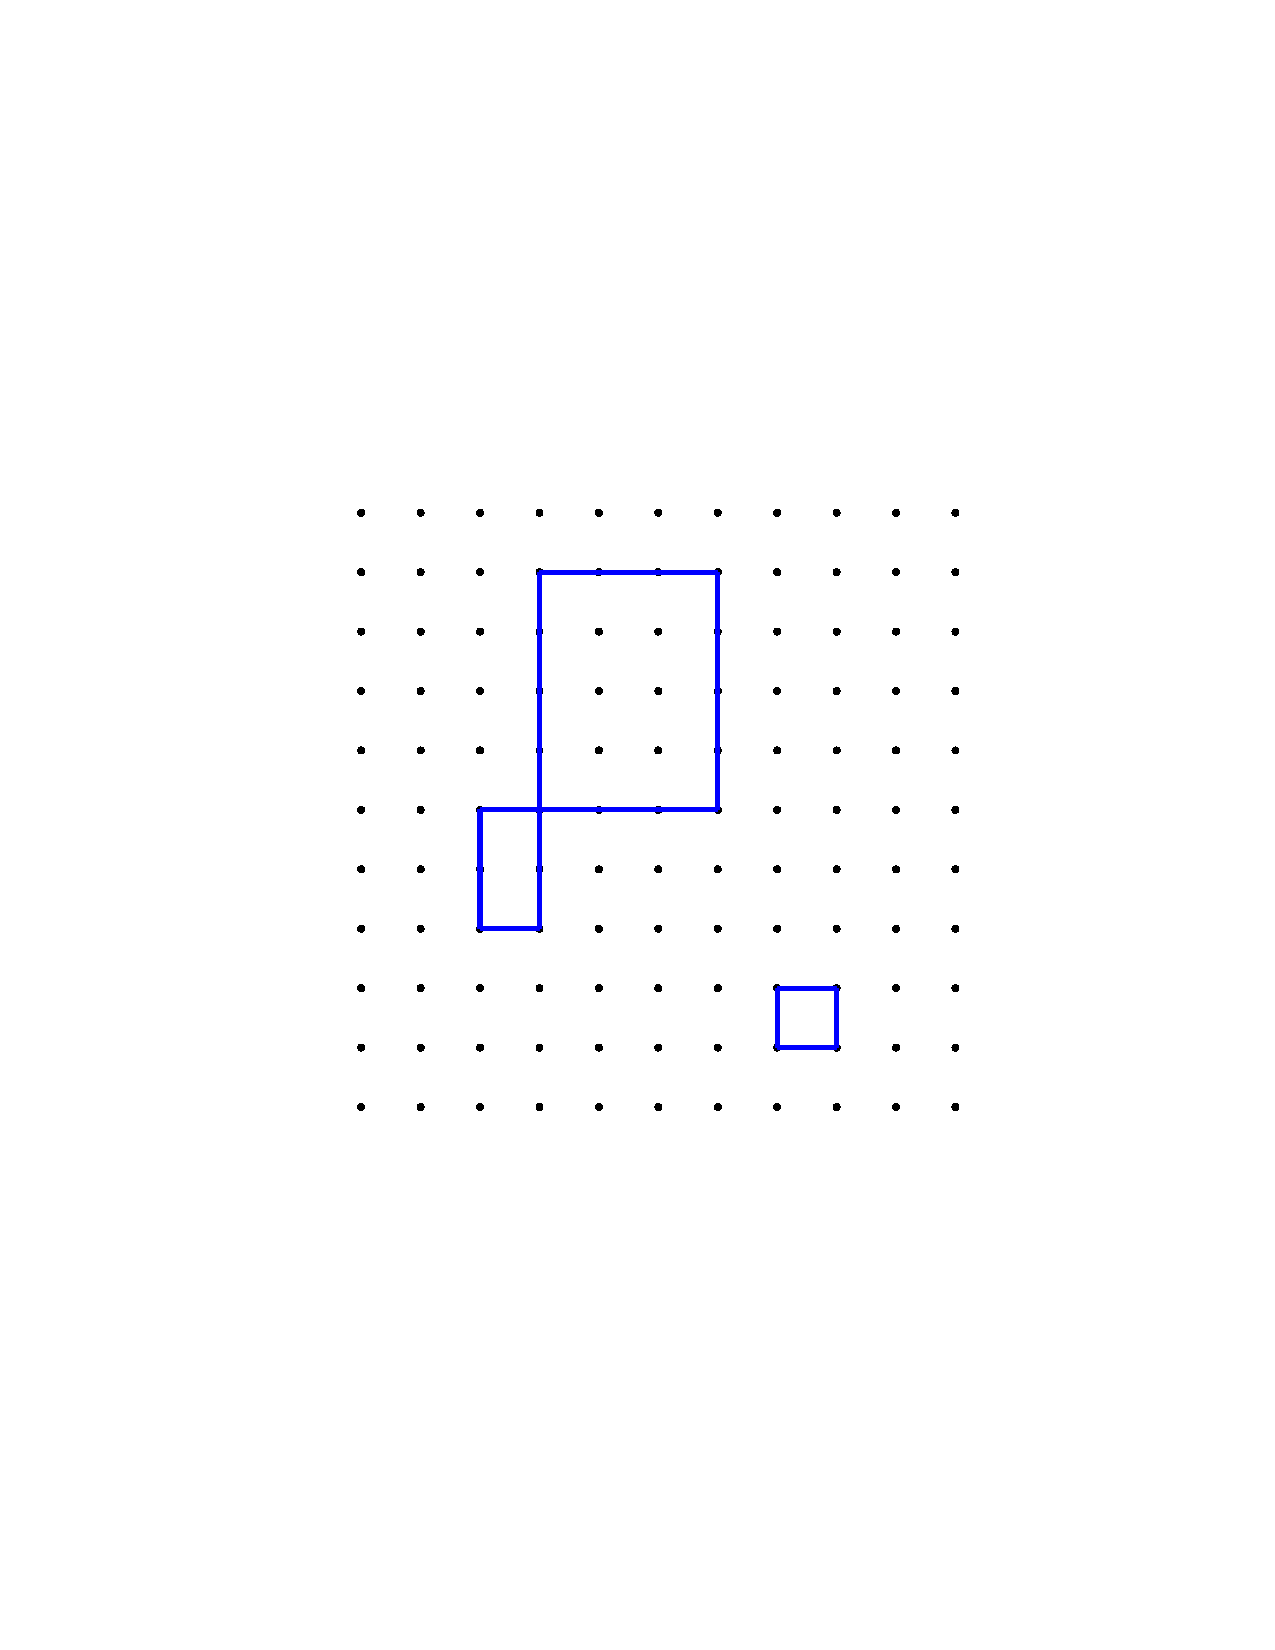
\includegraphics[width=0.49\textwidth]{graph_allowed}} 
\subfigure[Forbidden graph.]{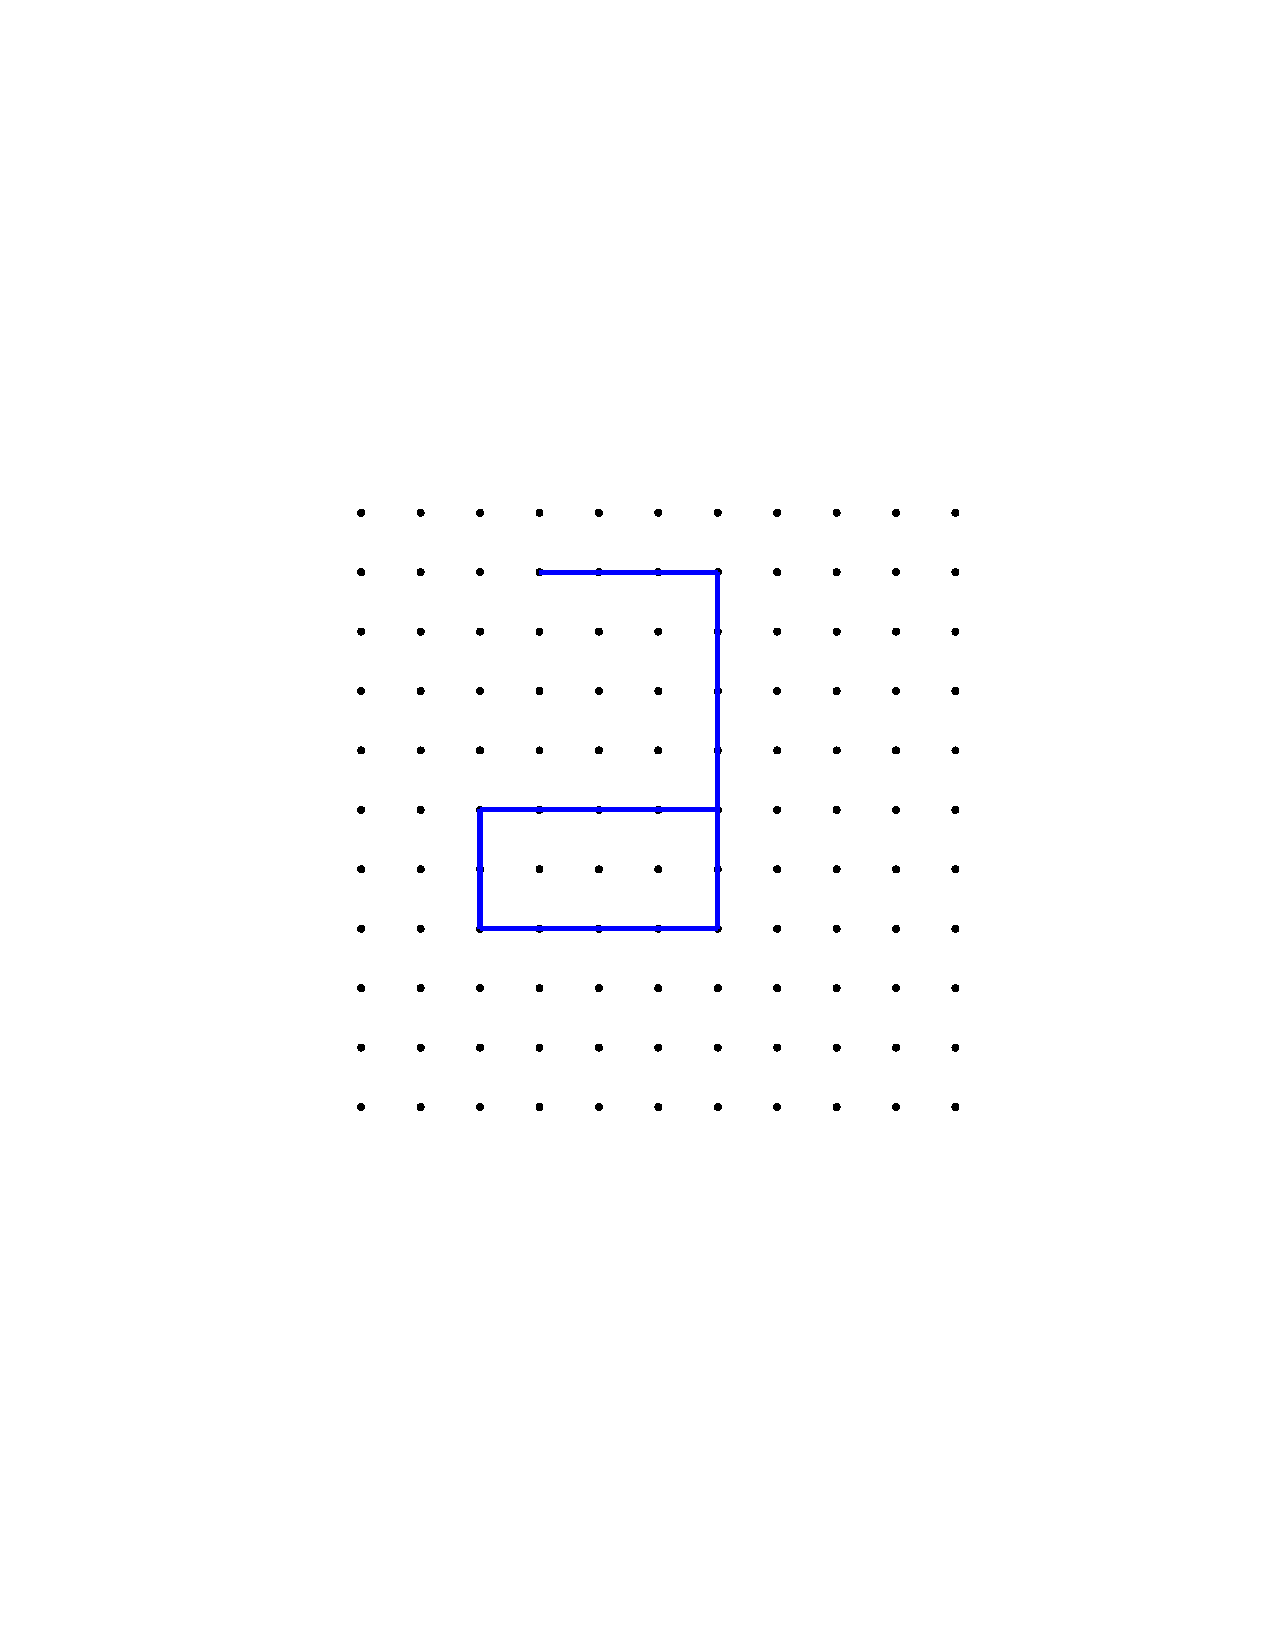
\includegraphics[width=0.49\textwidth]{graph_not_allowed}} 
\caption{{\it Graphical representation of the partition function of the Ising model.}\label{fig:graph:ising}}
\end{figure}
%
We can rewrite the sum over allowed graphs also in the form
\begin{align}\label{eq:ising:Z:g}
Z&=2^{N}\; \cosh^{2N}(j) \;\big(1+\sum_{n=4}^{\infty} g_{n}\;t^{n}\big)\;,
\end{align}
where $n$ is the number of edges and $g_{n}$ is the number of allowed graphs
with $n$ edges. We have already exploited that the smallest graph (besides the empty graph) has 4 edges.
Since each vertex has even order, the allowed graphs contain closed paths,
as can be seen in \fig{fig:graph:ising}. 



\subsection{Making the graphs unique}
The figure also contains a {\em node}, 
i.e. a vertex of order 4. Let's  try to draw the graph with a pencil on a piece of 
squared paper. We start at an arbitrary  vertex of order 2 and draw a line to one of the two connected vertices. If the next vertex also has order 2, it is obvious how to continue the drawing. When we reach a node, however, we have 3 options to continue:
{\it turn left, go straight, turn right}. 
It will turn out to be advantageous, to replace the graph by objects that allow to draw them in a unique way. Therefore, we will introduce graphical objects, that make a node unique. To this end a node is split into the three graphical objects, shown in
\fig{fig:ising:junction}.
%
\begin{figure}[h]
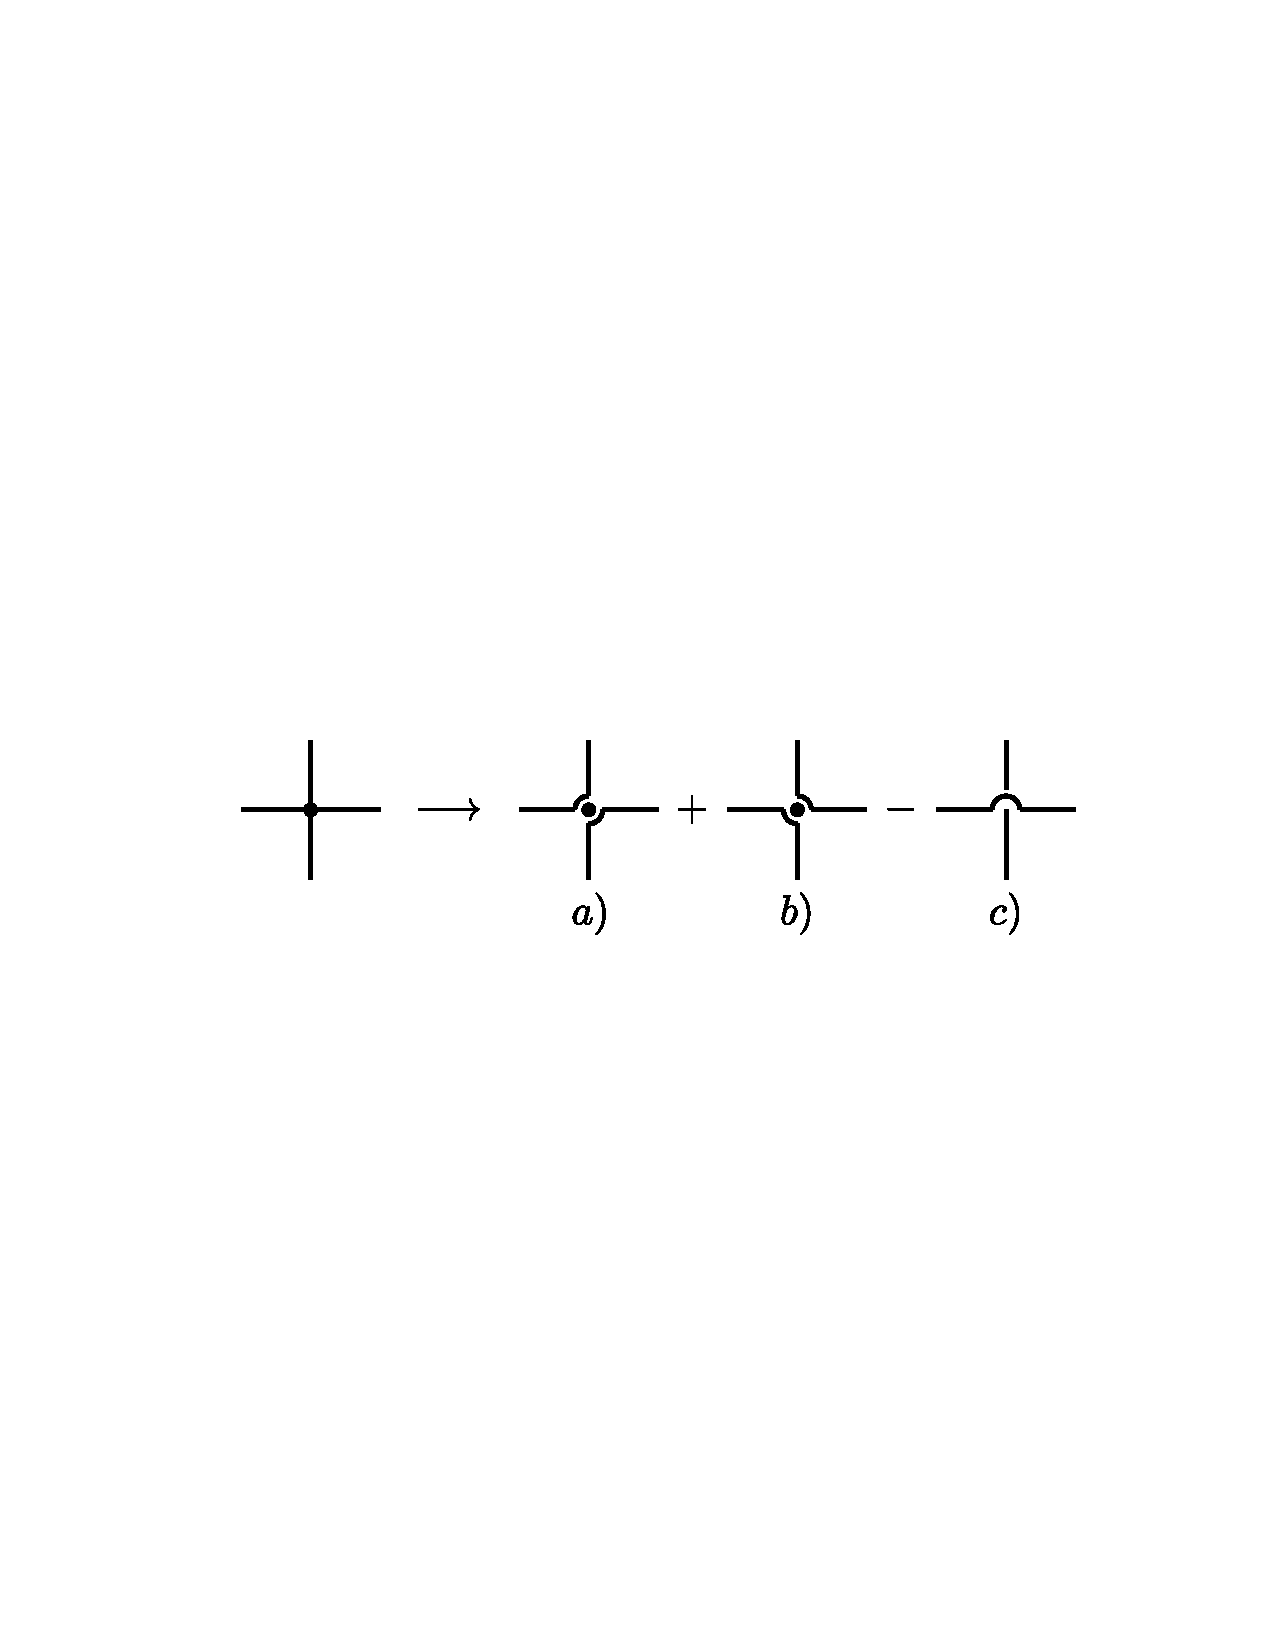
\includegraphics[width=1\textwidth]{junction}
\caption{{\it Splitting of a node with corresponding weights.}\label{fig:ising:junction}}
\end{figure}
%
This splitting  results in $3^{N_{n}}$
different new graphs, obtained from a graph with $N_{n}$ nodes. This would increase $g_{n}$ in a complicated way. To avoid this complication,
each new graphical element obtains a weight factor $\pm 1$, a shown in \fig{fig:ising:junction}. Now the three contributions of each node add up to $1$ again and the total count does not change.
The new graphs are denoted by $\tilde G$. They consist of one or more loops. 
As a remainder, a  {\em loop} (with e.g. $n$ edges) is a simply connected set  of edges, i.e. an object that can be drawn by starting at an arbitrary vortex on the loop, following the edges, and returning at the starting point after $n$ steps. The shortest loop has $4$ edges and the number of edges is always even.
In the new graphs $\tilde G$, the number of edges has not changed,   as compared to the  original graph,  but it has an extra weight factor
%
\begin{align*}
w(\tilde G) &= \big( -1 \big)^{N_{c}(\tilde G)}\;,
\end{align*}
%
where $N_{c}(\tilde G)$ stands for the number of \blue{crossings} ( decomposition c in \fig{fig:ising:junction}) of a graph $\tilde G$ of the new type.
By now $g_{n}$ is 
%
\begin{align*}
g_{n} &= \sum_{\tilde G}^{N_{e}(\tilde G)=n} \big( -1 \big)^{N_{c}(\tilde G)}\;.
\end{align*}
%

\subsection{Decomposing graphs into loops}
%
We are still not able to calculate the sum of all graphs analytically.
To this end we need to transform the graphs further.
Each graph $\tilde G$ with $n$ edges consists of  one or more loops,
which in total have $n$ edges. If a particular graph $\tilde G$ consists of $l$ loops,
we can devide the total weight between the loops. A loop $L$ contributes
a factor
%
$(-1)^{N_{c}(L)}\;$,
%
where $N_{c}(L)$ is the number of crossings in loop $L$.
The total weight is the product of the weights of the loops of  which the graph is formed.
Clearly, there is a one-to-one correspondence between all graphs $\tilde G$
with $n$ edges and all sets of loops with a total number $n$ of edges.
We define 
%
\begin{align}\label{eq:ising:def:D}
D_{l} &=
\begin{cases}
 \sum_{L}^{\text{loops with $l$ edges}}  \big( -1 \big)^{N_{c}(L)}&\text{if $l$ is even}	\\
 0&\text{otherwise}
\end{cases}\;.
\end{align}
%

Hence for $n\ge 4$ we may think that we can decompose $g_{n}$ into the contribution
of the loop decomposition:
%
\begin{align}\label{eq:ising:g:D}
g_{n}=\sum_{\tilde G} \delta_{N_{n}(\tilde G)=n} \;\big( -1 \big)^{N_{c}(\tilde G)}
&= \sum_{m=1}^{\infty} \frac{1}{m!} \sum_{l_{1}\ldots l_{m}=4}
\delta_{\sum_{\nu=1}^{m}l_{\nu} = n}
\prod_{\nu=1}^{m}
  D_{l_{\nu}}
\end{align}
%
Here $m$ is the number of loops and $l_{\nu}$ stands for the number of edges of loop $\nu$ and $D_{l_{v}}$ is the  corresponding weight obtained by summing over all realizations of a loop with $l_{\nu}$ edges. 
The factor $1/m!$ is required as the right hand sight creates a particulcar set of $m$
loops in $m!$ different permutations.
We can insert \eq{eq:ising:g:D} in \eq{eq:ising:Z:g} and obtain
%
\begin{align*}
\sum_{n=4}^{\infty} g_{n} t^{n}&=
\sum_{m=1}^{\infty} \frac{1}{m!} \sum_{l_{1}\ldots l_{m}=4}
 \underbrace{\sum_{n=4}^{\infty}
 \delta_{\sum_{\nu=1}^{m}l_{\nu} = n }
}_{\color{blue} = 1}
\prod_{\nu=1}^{m}
  D_{l_{\nu}} t^{l_{\nu}}\\
  &=
\sum_{m=1}^{\infty} \frac{1}{m!} 
\prod_{\nu=1}^{m}
\bigg(\sum_{l=4}  D_{l} t^{l}\bigg)\\
  &=
\sum_{m=1}^{\infty} \frac{1}{m!} 
\bigg(\sum_{l=4}  D_{l} t^{l}\bigg)^{m}\\
&=\exp\bigg( \sum_{l=4}  D_{l} t^{l} \bigg)-1
\end{align*}
%
Hence according to \eq{eq:ising:Z:g} we have
%
\begin{align}\label{eq:ising:ln:Z}
\ln(Z) &= N \ln(2) + 2N \ln\big(\cosh(j)\big) + \sum_{m=1}^{\infty}  D_{m} t^{m} \;.
\end{align}
%
%
\begin{figure}[t]
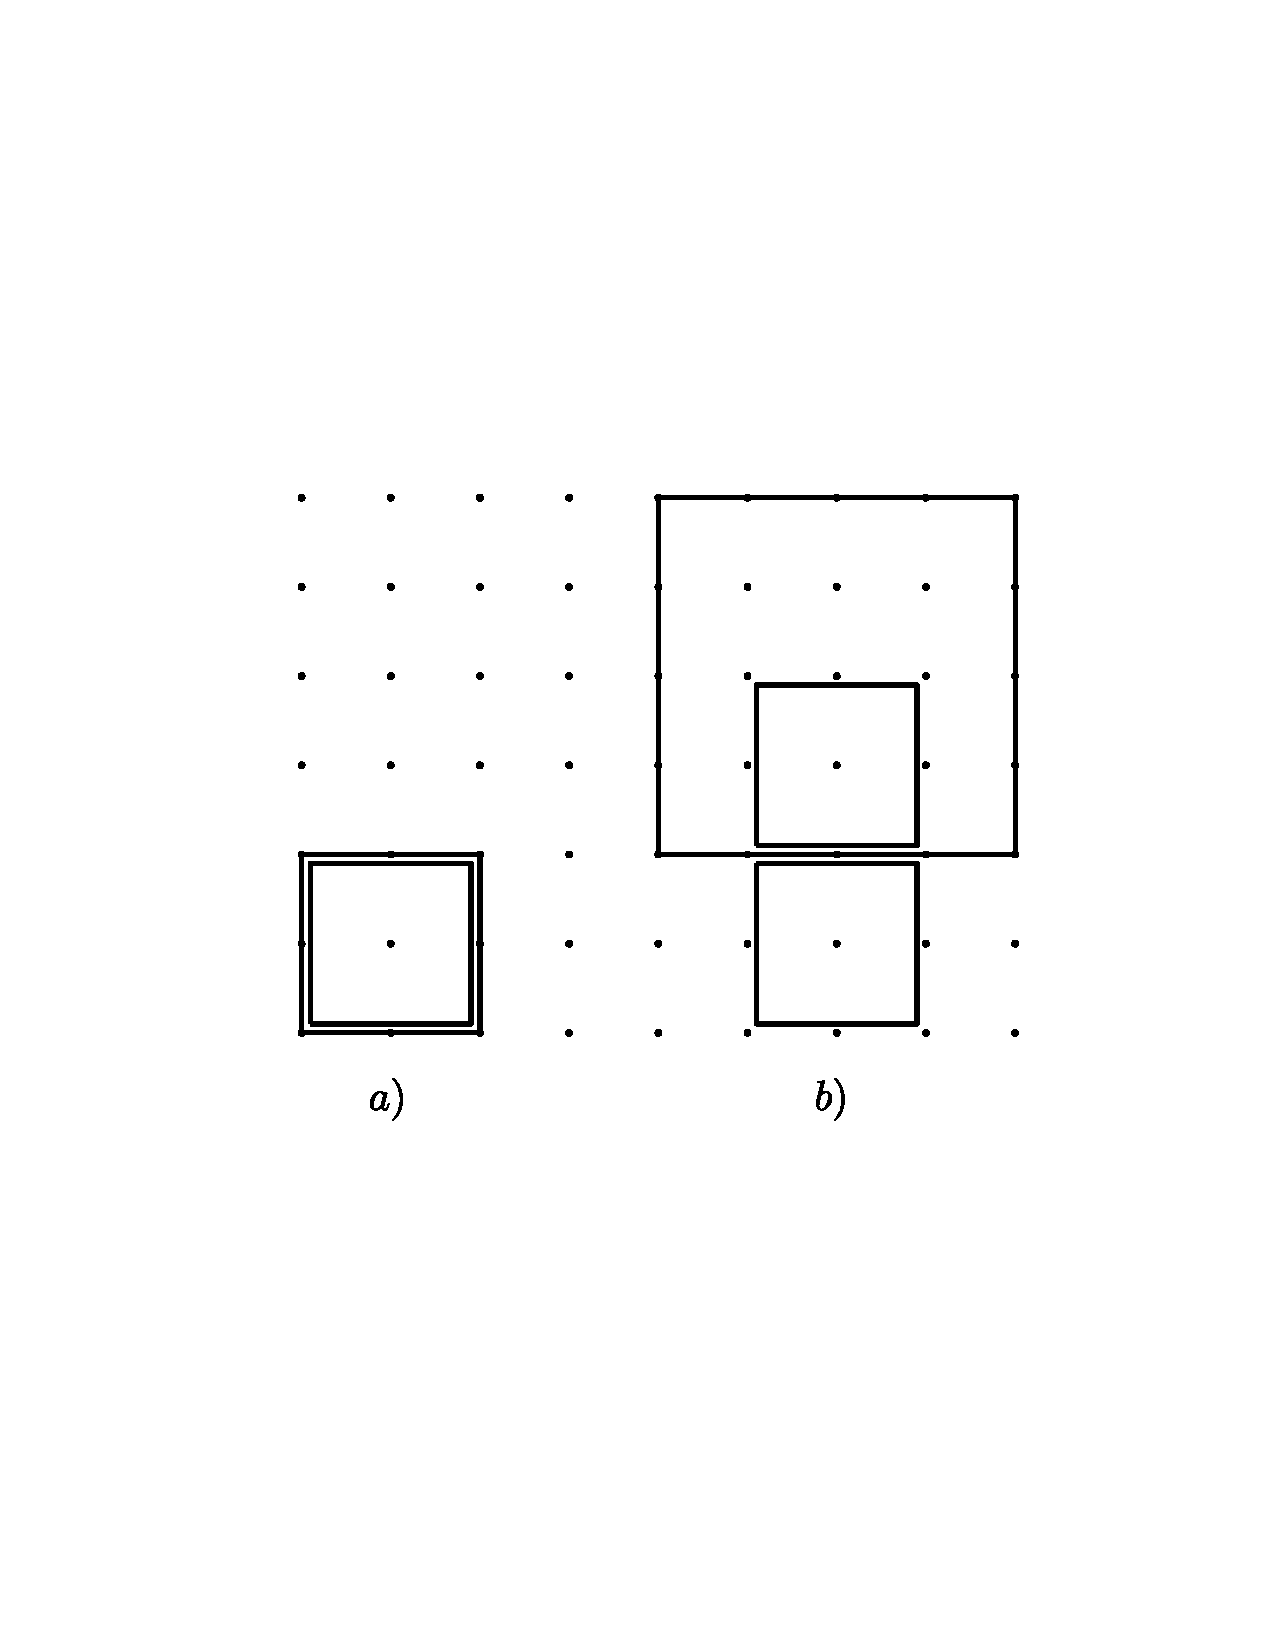
\includegraphics[width=.8\textwidth]{ising_crossings}
\caption{{\it Examples of configurations that occur if loops are placed independently. Such configurations are no valid graphs $\tilde G$.}\label{fig:ising:crossings}}
\end{figure}
%
The sum can start at $m=1$ (instead of $m=4$) since \eq{eq:ising:def:D} counts loops and the shortest loop has length $4$ anyways.
However, \eq{eq:ising:g:D} is not really correct. On the rhs the sum runs over all configurations
of independently arranged loops. I.e. there will be configurations where edges occur more than once, like in \fig{fig:ising:crossings}. Such a configuration is not included in $\tilde G$.
%
\begin{figure}[t]
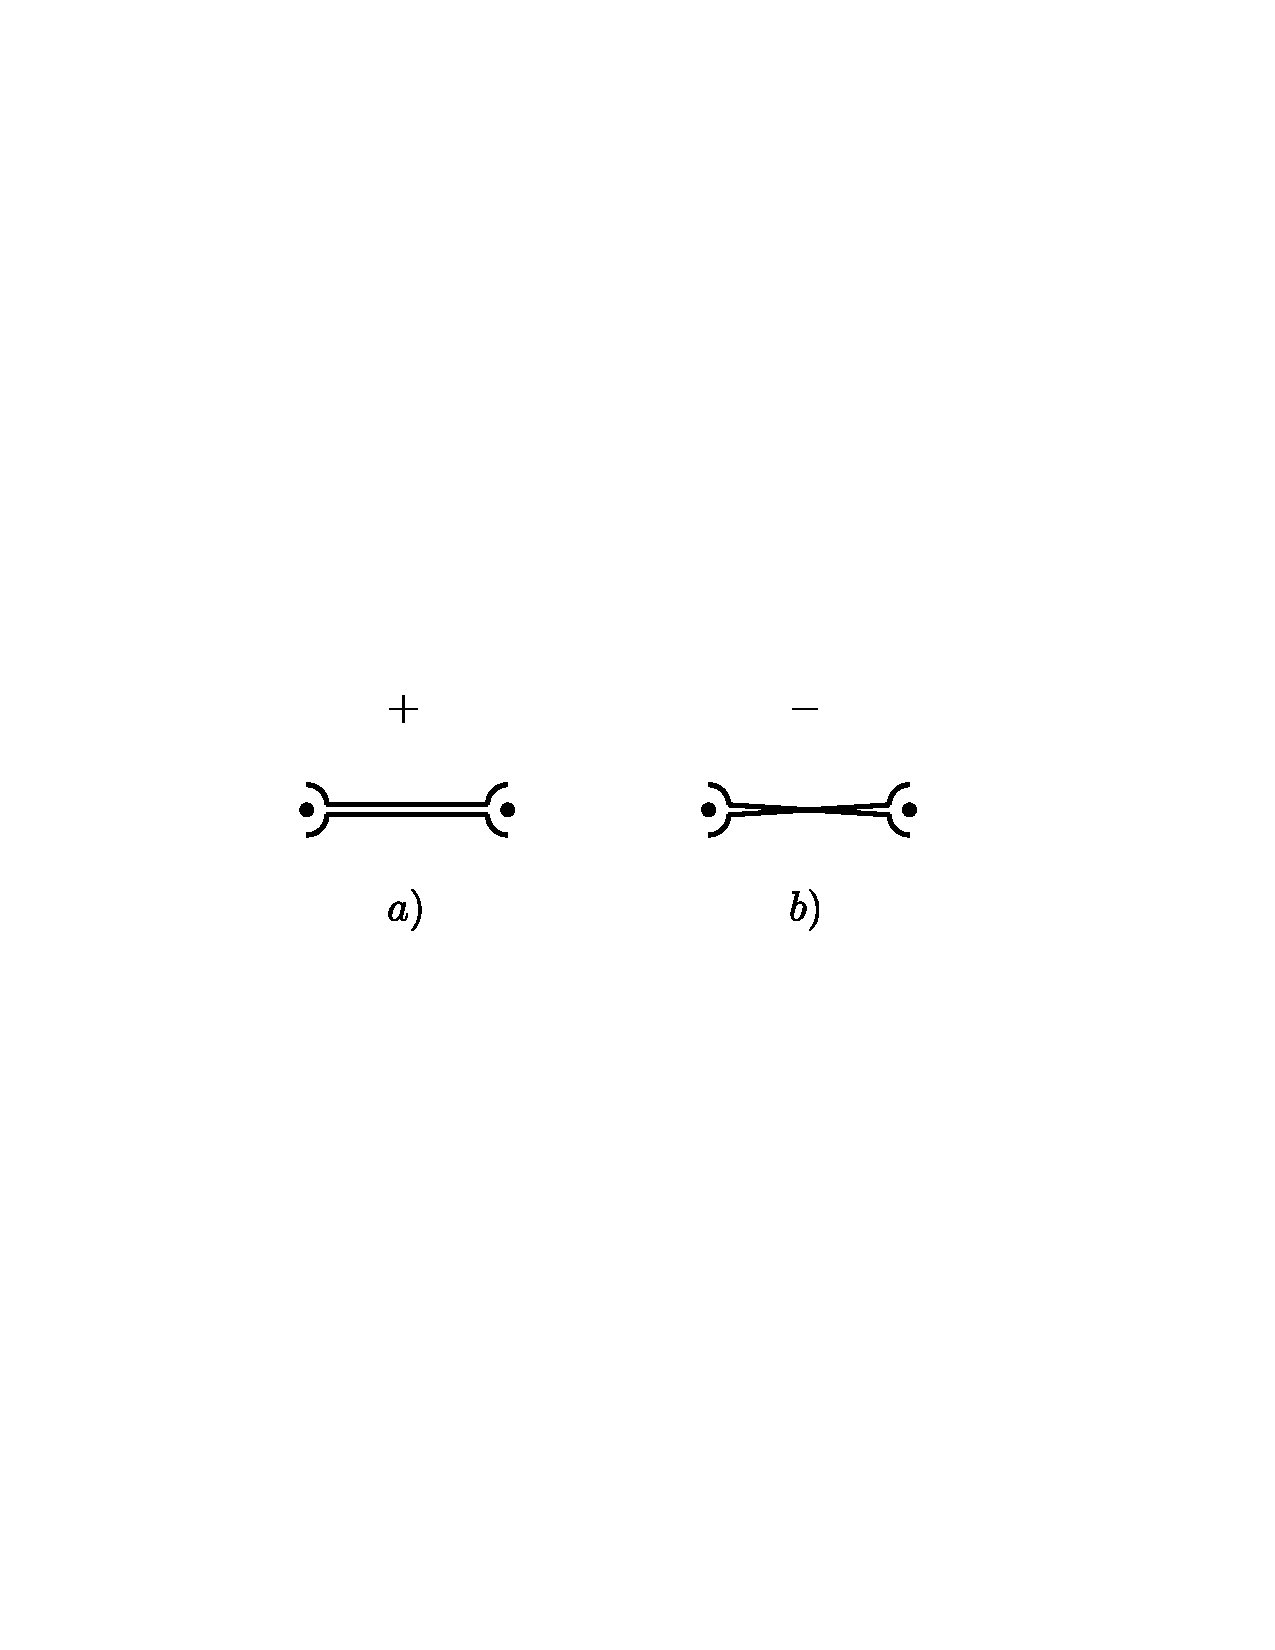
\includegraphics[width=.8\textwidth]{double_bonds}
\caption{{\it Double occupied edges.}\label{fig:ising:double:bonds}}
\end{figure}
%
However, there is a very simple cure. We allow such configurations also in $\tilde G$, but in addition to double bonds, say, as in  \fig{fig:ising:crossings} a) or schematically depicted in \fig{fig:ising:double:bonds} a)
we also include configurations that occur if we cross the lines as shown  in \fig{fig:ising:double:bonds} b) and give them a weight $-1$. 
The sum of these configurations adds up to zero.
The same holds true, if there are threefold
edges as in \fig{fig:ising:crossings} b) or even $m$-fold edges. Generally, in the case of $m$-fold edges there are $m!$ possible connections (permutations) of the incoming and outgoing lines. The number of crossings is even/odd  if the permutation is even/odd. As the number of even permutations is always equal to the number of odd permutations, the signs add up to zero.
In the case of \fig{fig:ising:crossings} a) the new configurations are depicted in
\fig{fig:ising:crossings:new}.
%
\begin{figure}[t]
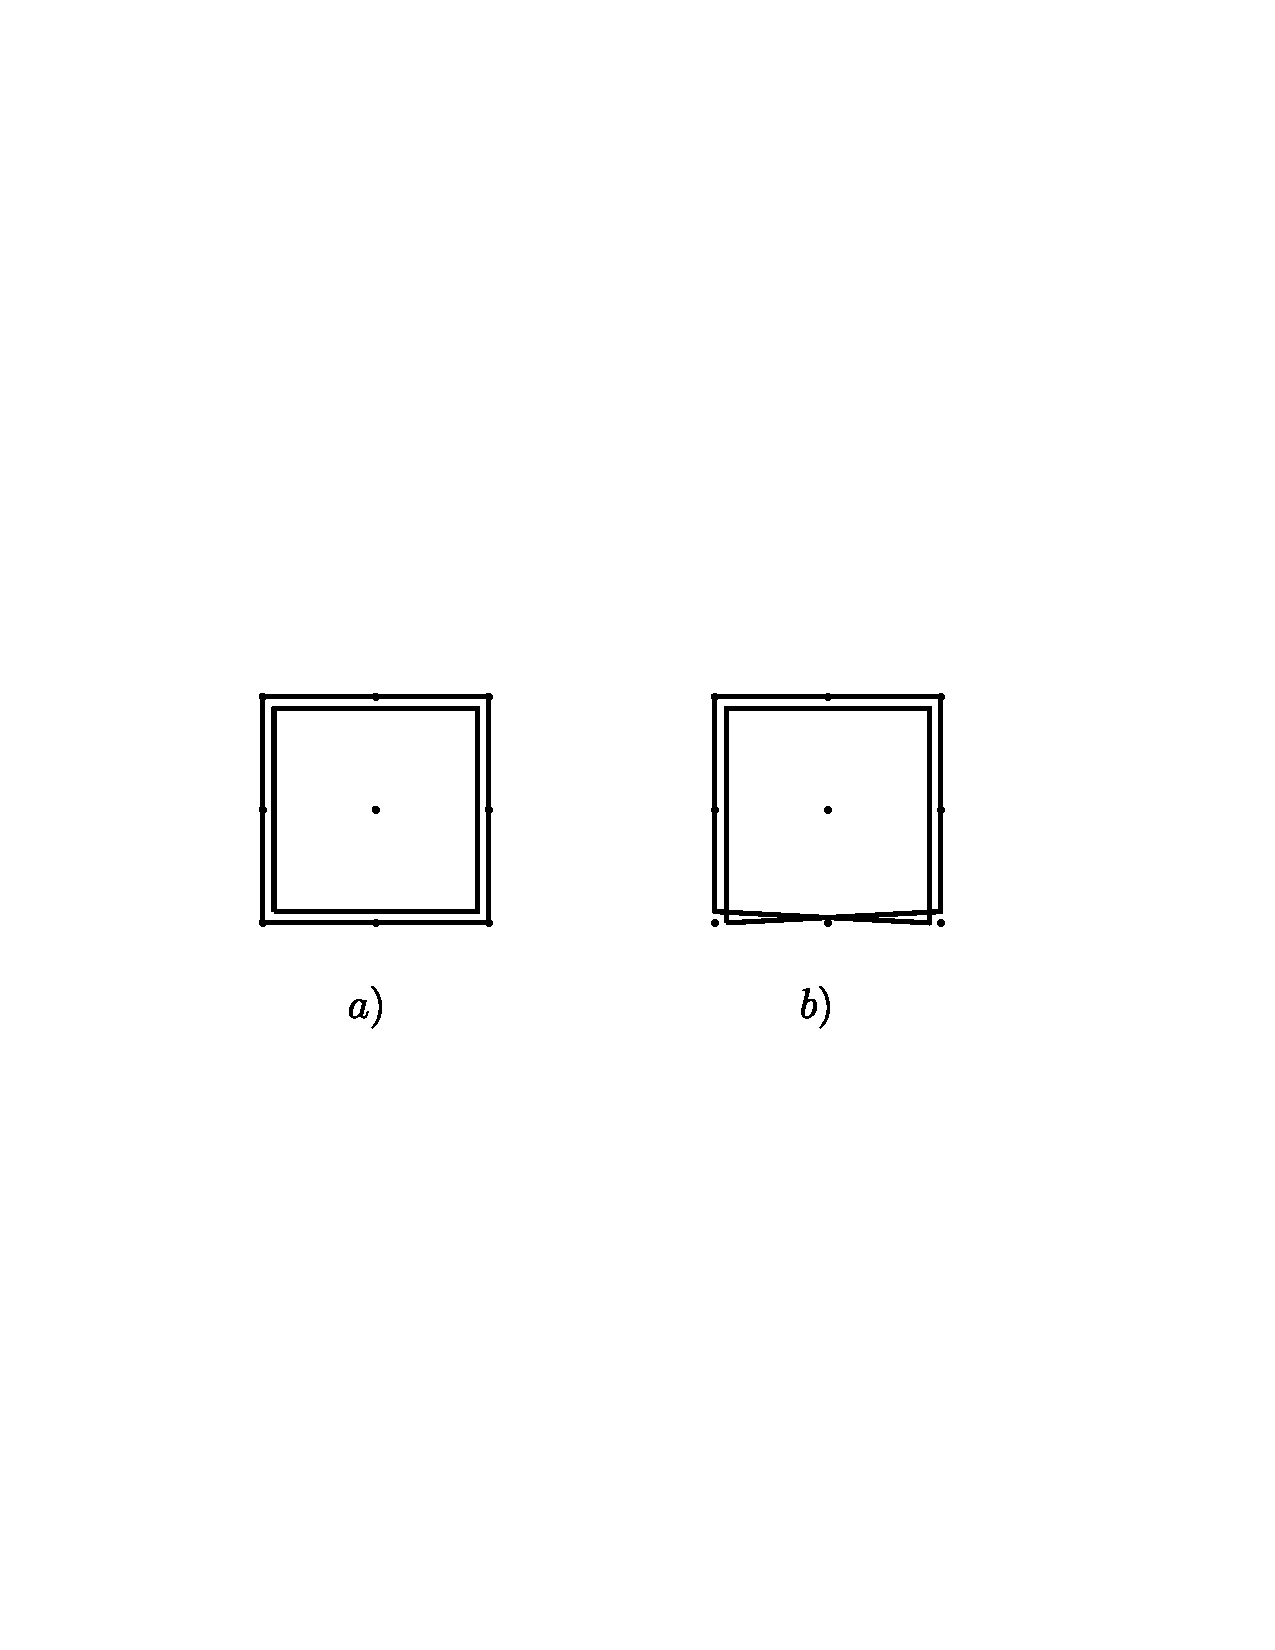
\includegraphics[width=.8\textwidth]{ising_crossings_new}
\caption{{\it Double occupied edges.}\label{fig:ising:crossings:new}}
\end{figure}
%
Now a) represents a double loop generated by placing loops independently, while b)
shows a single loop, which is passed twice. Including b) in the allowed single loops
ensures the cancelation of forbidden configurations generated by placing loops independently.
The same holds true for even more complex structures, such as tripple loops.

If we include the new type of crossings in the loops, then the previous formulas
 (\eq{eq:ising:def:D} and \eq{eq:ising:ln:Z})  remain unchanged, with the exception that these crossings also contribute to the number of crossings.
 
 

 \subsubsection{Counting then number of loops and corresponding crossing}
The remaining task is the determination of $D_{l}$, which includes the task of counting the crossings. To this end we introduce directed paths. The n-th step of the path is encoded in
%
\begin{align}
S^{(n)} &=\big( \vv x^{(n)}, \vv d ^{(n)}\big)\,
\end{align}
%
where $\vv x^{(n)}$ represents the initial site of the n-th step, 
and $\vv d^{(n)}\in\{\pm\vv e_{x},\pm\vv e_{y}\}$ 
the direction of the n-th step.  
A {\em path} from $S^{(0)}$ to $S^{(m)}$ is defined by the sequence
%
\begin{align*}
{\cal P}&=S^{(0)},S^{(1)},\ldots,S^{(m)}
\end{align*}
%
Clearly, we have the condition
%
\begin{align}\label{eq:ising:path:cond}
\vv x^{(n+1)} &=\vv x^{(n)} + \vv d^{(n)}\;.
\end{align}
%
As the allowed loops do not contain elements that occur when $\vv d^{(n+1)}=-\vv d^{(n)}$,
we omit such steps. We define the weight of such a path as
%
\begin{align}
w ({\cal P}) &= \prod_{l=1}^{m}e^{i \tfrac{1}{2}\Phi(\vv d^{(l-1)},\vv d^{(l)})}\;,
\end{align}
%
where $\Phi(\vv d, \vv d')$ is the angle between the vectors $\vv d$ and $\vv d'$, defined as follows.
%
\begin{align}\label{eq:}
\Phi(\vv d,\vv d') &=
\begin{cases}
	0&\text{if } \vv d , \vv d' \text{are parallel}\\
	\frac{\pi}{2}&\text{if } \vv d' \text{ is anti-clockwise rotated from } \vv d\\
		-\frac{\pi}{2}&\text{if } \vv d' \text{ is clockwise rotated from } \vv d\\
		\text{forbidden}&\text{if } \vv d , \vv d' \text{ are anti-parallel}
\end{cases}
\end{align}
%
\begin{figure}[t]
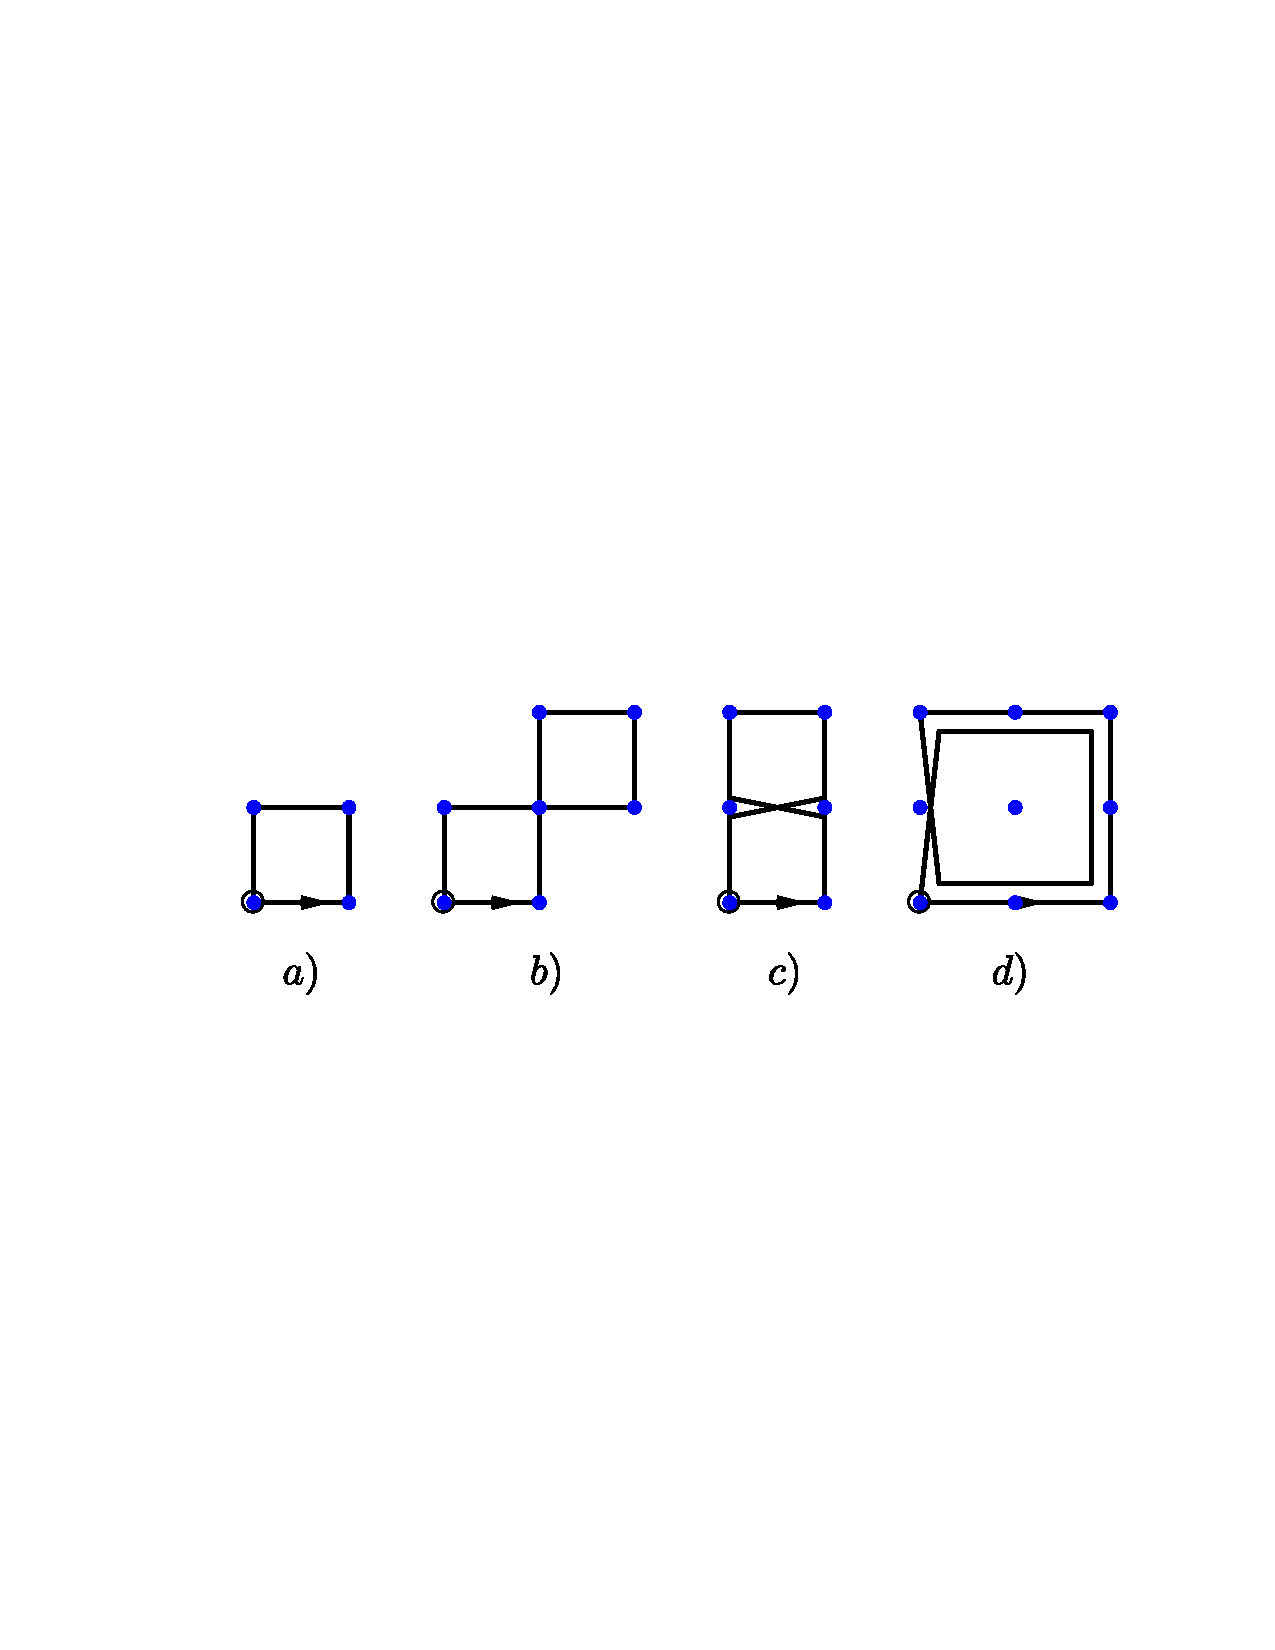
\includegraphics[width=.8\textwidth]{ising_paths}
\caption{{\it Representative paths and weights.}\label{fig:ising:paths}}
\end{figure}
%
In \fig{fig:ising:paths} some examples of allowed loops (paths) are given, for which we want to compute the weight. We start at the lower left corner and follow the arrow. 
We recall that turning left at a vertex gives $+\tfrac{\pi}{2}$, a right turn $-\tfrac{\pi}{2}$
and crossing straight adds zero.
In subfigure a)
the 4 angles $\Phi$ encountered during the path are all $\pi/2$. The four angle add up to $2 \pi$.
In other words we have performed four left turns
The weight is then
%
\begin{align*}
w &=e^{i \tfrac{1}{2} 2\pi} = -1\;.
\end{align*}
% 
For example b) the angles are in units of $\tfrac{\pi}{2}$: $1,0,-1,-1,-1,0,1,1$, with a sum of $0$ and a weight $w=+1$. In other words the number of left and right turns is equal. That is also the case in subfigure c). In example d) a loop is twice passed, so the total angle is $4 \pi$ and a phase factor $+1$.
We find in all  cases
%
\begin{align*}
w({\cal P}) &= - (-1)^{N_{c}(L)}\;,
\end{align*}
%
which is the required weight in \eq{eq:ising:def:D} apart from a global minus sign.

Now we define a matrix ${\cal M}$ with matrix elements
%
\begin{align*}
\bra{S'} M_{m}\ket{S} = \text{sum of the weights of all paths from $S$  to $S'$  in $m$ steps}\;.
\end{align*}
%
The value of the matrix element is zero, if there is no path connecting $S$ and $S'$
in $m$ steps.
For $m=m_{1}+m_{2}$  we have  by definition
%
\begin{align*}
\bra{S'} M_{m}\ket{S}  &=
\sum_{S''}\bra{S'} M_{m_{1}}\ket{S''} \bra{S''} M_{m_{2}}\ket{S}   \;,
\end{align*}
%
which is the common matrix product. Consequently, we have
%
\begin{align*}
{\cal M} _{m}  &= \big({\cal M}_{1}\big)^{m}\;.
\end{align*}
%
${\cal M}_{1}$ has the dimension $4 N\times 4N$, as each step $S=(\vv x,\vv d)$ has
$N$ possible sites $\vv x$ and 4 possible directions $\vv d$. Most of the matrix elements, however, are zero. The fact that a path cannot be retraced is also accounted for in ${\cal M}_{1}$.

We can now easily express the sought-for weight  $D_{m}$ as
%
\begin{align*}
D_{m} &= - \frac{1}{2m}\sum_{S} \bra{S} {\cal M}_{m} \ket{S}
= -\frac{1}{2m} \tr{{\cal M}_{1}^{m} }
\end{align*}
%
\emphasize{prove}{
\begin{enumerate}
	\item The trace is required to sum over all initial vertices of the loop and to make sure that the loop is really closed
	\item Since each vertex of a loop occurs as initial point in the trace, we have to divide by $m$
	\item Each loop can be traversed in two direction, which explains the factor $1/2$.
	\item The minus sign has been expained before.
\end{enumerate}
}
In total we therefore have according to \eq{eq:ising:ln:Z}
\begin{align*}
\ln(Z) &= N \ln(2) +2 N \ln\big(\cosh(j)\big) + \sum_{m=1}  D_{m} t^{m} \\
&= N \ln(2) + 2 N \ln\big(\cosh(j)\big)  - \frac{1}{2}\tr{\sum_{m=1} \frac{\big(t{\cal M}_{1}\big)^{m}}{m} }\\
&= N \ln(2) + 2 N \ln\big(\cosh(j)\big)  + \frac{1}{2}\tr{\ln\big(\mathbf 1-t{\cal M}_{1}\big)}\\
&= N \ln(2) + 2 N \ln\big(\cosh(j)\big)  + \frac{1}{2}\ln\text{det}\big[\big(\mathbf 1-t{\cal M}_{1}\big)\big]\;.
\end{align*}

As said before, the size of the matrix ${\cal M}_{1}$ is $4N\times 4N$. The matrix elements are defined via
%
\begin{align*}
\bra{\vv  x,\vv d} {\cal M}_{1}\ket{\vv x',\vv d'}\;.
\end{align*}
%
Since we use pbc, it is advantageous to perform a Fourier transform with respect to $\vv x$ and 
$\vv x'$. The determinant is invariant against such a unitary transformation. Moreover, due to
translational invariance of the problem, we obtain
%
\begin{align*}
\bra{\vv  q,\vv d} {\cal M}_{1}\ket{\vv q',\vv d'}&=
\frac{1}{N}\sum_{\vv x,\vv x'} e^{-i\big(\vv x\cdot \vv q-\vv x'\cdot \vv q'\big)}
\bra{\vv 0,\vv d} {\cal M}_{1}\ket{\underbrace{\vv x'-\vv x}_{\Delta\vv  x},\vv d'}\\
&= \underbrace{
\frac{1}{N}\sum_{\vv x} e^{-i\vv x\cdot (\vv q-\vv q')}
}_{\color{blue} = \delta_{\vv q\vv q'}}\sum_{\Delta\vv x} e^{i \vv q'\cdot\Delta \vv x}
\bra{\vv 0,\vv d} {\cal M}_{1}\ket{\Delta\vv  x,\vv d'}\\
&= \delta_{\vv q\vv q'}\;\sum_{\Delta\vv x} e^{i \vv q\cdot\Delta \vv x}
\bra{\vv 0,\vv d} {\cal M}_{1}\ket{\Delta\vv  x,\vv d'}\;.
\end{align*}
%
According to \eq{eq:ising:path:cond} we have the condition 
%
\begin{align*}
\vv x' &= \vv x +\vv d\\
\Rightarrow\qquad \Delta \vv x &= \vv x' -\vv x = \vv d\;.
\end{align*}
%
Hence the $4\times 4$ matrix $M(\vv q)$ hat the matrix elements
%
\begin{align*}
\bra{\vv  q,\vv d} {\cal M}_{1}\ket{\vv q',\vv d'}
&= \delta_{\vv q\vv q'}\; 
e^{i \vv q\cdot\vv d}\;
\bra{\vv 0,\vv d} {\cal M}_{1}\ket{\vv d,\vv d'}\\
&= \delta_{\vv q\vv q'}\; 
\underbrace{
e^{i \vv q\cdot\vv d}\;
e^{i\frac{1}{2}\Phi(\vv d,\vv d')}
}_{\color{blue} = M_{\vv d,\vv d'}}\\
\end{align*}
%
The inverse transformation is
%
\begin{align*}
\bra{\vv  x,\vv d} {\cal M}_{1}\ket{\vv x',\vv d'}&=\frac{1}{N}
\sum_{\vv q} e^{i\big(\vv x-\vv x')\cdot \vv q }
\bra{\vv q,\vv d} {\cal M}_{1} \ket{\vv q,\vv d'}\;,
\end{align*}
%
and, therefore, 
%
\begin{align*}
\bra{\vv  x,\vv d} {\cal M}^{n}\ket{\vv x',\vv d'}&=\frac{1}{N}
\sum_{\vv q} e^{i\big(\vv x-\vv x')\cdot \vv q }
\bra{\vv q,\vv d} ({\cal M}_{1})^{n} \ket{\vv q,\vv d'}\\
&=\frac{1}{N}
\sum_{\vv q} e^{i\big(\vv x-\vv x')\cdot \vv q }
\bigg(\big( M(\vv q) \big)^{n}\bigg)_{\vv d,\vv d'}\;.
\end{align*}
%

The remaining  $4\times 4$ matrix $M(\vv q)$ has the matrix elements
%
%
%\begin{center}
%M:
% \begin{tabular}{||c|c c c c||} 
% \hline
% $\vv d \backslash  \vv d' $&$\vv e_{x}$ & $\vv e_{y}$ & $-\vv e_{x}$  &$-\vv e_{y}$ \\ [0.5ex] 
% \hline\hline
%$\vv e_{x}$  &$e^{iq_{1}}$& $\lambda e^{i q_{1}}$& $0$ & $\lambda^{*}e^{iq_{1}}$ \\ 
% \hline
% $\vv e_{y}$&$\lambda^{*} e^{i q_{2}}$& $e^{iq_{2}}$ & $\lambda e^{i q_{2}}$  & $0$ \\
% \hline
%$-\vv e_{x}$ &$0$ & $\lambda^{*} e^{-i q_{1}}$& $e^{-iq_{1}}$  & $\lambda e^{-i q_{1}}$ \\
% \hline
%$-\vv e_{y}$ &$\lambda e^{-i q_{2}}$& $0$  &$\lambda^{*} e^{-i q_{2}}$ & $e^{-iq_{2}}$ \\[1ex] 
% \hline
%\end{tabular}
%\end{center}
%
\begin{center}
$M(\vv  q)$:
 \begin{tabular}{||c|c c c c||} 
 \hline
 $\vv d \backslash  \vv d' $&$\vv e_{x}$ & $-\vv e_{x}$ & $\vv e_{y}$  &$-\vv e_{y}$ \\ [0.5ex] 
 \hline\hline
$\vv e_{x}$  &$e^{iq_{1}}$& $0$& $\lambda e^{i q_{1}}$ & $\lambda^{*}e^{iq_{1}}$ \\ 
\hline
$-\vv e_{x}$ &$0$ & $e^{-iq_{1}}$& $\lambda^{*} e^{-i q_{1}}$  & $\lambda e^{-i q_{1}}$ \\
 \hline
 $\vv e_{y}$&$\lambda^{*} e^{i q_{2}}$& $\lambda e^{i q_{2}}$ & $e^{iq_{2}}$  & $0$ \\
 \hline
$-\vv e_{y}$ &$\lambda e^{-i q_{2}}$  &$\lambda^{*} e^{-i q_{2}}$& $0$ & $e^{-iq_{2}}$ \\[1ex] 
 \hline
\end{tabular}
\end{center}
%

with the definition $\lambda=e^{i\tfrac{\pi}{4}}$.
This can also be written as
%
\begin{subequations}\label{eq:}
\begin{align}
M(\vv q) &=  D(\vv q) \tilde M\\
D(\vv q) &=\text{diag} \big[ e^{i q_{1}},e^{-i q_{1}},e^{i q_{2}} ,e^{-i q_{2}}\big]\\
\tilde M &=
\begin{pmatrix}
	1&0&\lambda,\lambda^{*}\\
		0&1&\lambda^{*},\lambda\\
\lambda^{*},\lambda&	1&0&\\
\lambda,\lambda^{*}&	0&1&
\end{pmatrix}
\end{align}
\end{subequations}
%
Here $\tilde M$ is a hermitean matrix bat $M$ is not.
As the matrix is blockdiagonal in $\vv q$, $\vv q'$ we have
%
\begin{align*}
\text{det} \big(\mathbf 1- t {\cal M}_{1} \big)=\text{det} \big(t {\cal M}_{1} - \mathbf 1 \big)
&=\prod_{\vv q}^{1bc} \det\big( t M(\vv q)  - \mathbf 1 \big)
\end{align*}
%
With $Q_{\alpha}=t e^{iq_{\alpha}}$ the matrix  argument of the determinant reads
%
%\begin{align*}
%  t M(\vv q) - \mathbf 1=
%\begin{pmatrix}
%Q_{1}-1& \lambda Q_{1}&0& \lambda^{*} Q_{1}\\
% \lambda^{*}Q_{2}&Q_{2}-1& \lambda Q_{2}&0\\
%0& \lambda^{*}Q_{1}^{*}&Q_{1}^{*}-1& \lambda Q_{1}^{*}\\
% \lambda Q_{2}^{*}&0& \lambda^{*}Q_{2}^{*}&  Q_{2}^{*}-1
%\end{pmatrix}
%\end{align*}
%%


%
\begin{align*}
  t M(\vv q) - \mathbf 1=
- \begin{pmatrix}
Q_{1}-1& 0& \lambda Q_{1}& \lambda^{*} Q_{1}\\
0& Q_{1}^{*}-1&\lambda^{*}Q_{1}^{*}& \lambda Q_{1}^{*}\\
\lambda^{*}Q_{2}&\lambda Q_{2}&Q_{2}-1& 0\\
 \lambda Q_{2}^{*}& \lambda^{*}Q_{2}^{*}& 0& Q_{2}^{*}-1
\end{pmatrix}\;.
\end{align*}
%
The determinant  yields (according to MATHEMATICA)

%
\begin{align*}
\ln
\bigg[
\det \big(
\mathbf 1- t {\cal M}_{1} 
\big)\bigg] &=\sum_{\vv q}^{1bz}
\ln
\bigg[ 
\big( 1+t^{2} \big)^{2}
-2t (1-t^{2}) 
\big( \cos(q_{1})+\cos(q_{2})
\big) 
\bigg]\;.
\end{align*}
%
Then the free energy per site is 
%
\begin{align}\label{eq:}
-\beta\frac{F}{N} &= \ln(2) + 2\ln(\cosh(j)) +\frac{1}{2N}\sum_{\vv q}^{1bc}
\ln\bigg[ \big( 1+t^{2} \big)^{2}-2t (1-t^{2}) \big( \cos(q_{1})+\cos(q_{2}) \big) \bigg]
\end{align}
%
We introduce the normalized density of states $\rho(\varepsilon)$ corresponding to the dispersion
%
\begin{align}\label{eq:ising:dispersion}
 \varepsilon(\vv q) &= - \big( \cos(q_{1})+\cos(q_{2} ) \big) \\
 \rho(\varepsilon) &= \frac{1}{N}\sum_{\vv q}^{1bc} \delta(\varepsilon(\vv q) - \varepsilon)
\end{align}
%
Then the free  energies reads
%
\begin{align}\label{eq:}
-\beta\frac{F}{N} &= \ln(2) + 2\ln(\cosh(j)) +\frac{1}{2}\int d\varepsilon \rho(\varepsilon)
\ln\big[ \big( 1+t^{2} \big)^{2}+2t (1-t^{2}) \;\varepsilon \big]\;.
\end{align}
%
Moreover, we use
%
\begin{align*}
\cosh(j) &=\frac{1}{\sqrt{1-t^{2}}}\;,\qquad \big(t:=\tanh(j)\big)\\
2 \ln\big(  \cosh(j)\big) &= \frac{1}{2}\ln\big( (1-t^{2})^{-2} \big)
= \frac{1}{2} \int d\varepsilon\; \rho(\varepsilon)  \ln\big(\big( 1-t^{2} \big)^{-2}\big)
\end{align*}
%
to obtain
\begin{align*}
-\beta\frac{F}{N} &= \ln(2) +\frac{1}{2}\int d\varepsilon \rho(\varepsilon)
\ln\bigg[ \bigg( \frac{1+t^{2}}{1-t^{2}} \bigg)^{2}+ \bigg(\frac{2t}{1-t^{2}}\bigg) \;\varepsilon\bigg]\\
&= \ln(2) +\frac{1}{2}\int d\varepsilon \rho(\varepsilon)
\ln\bigg[\underbrace{
 \bigg( \frac{1+t^{2}}{1-t^{2}} \bigg)^{2}-  \bigg(\frac{4t}{1-t^{2}}\bigg)
}_{\color{blue} = \big( 1-\sinh(2j) \big)^{2}}+ \underbrace{
\bigg(\frac{2t}{1-t^{2}}\bigg)
}_{\color{blue} = \sinh(2j)} \;(2+\varepsilon) \bigg]\;.
\end{align*}
%
%
\emphasize{proof}{
%
\begin{align*}
\frac{2 t}{1-t^{2}} &=\frac{2 \tanh(j)}{1-\tanh^{2}(j)}\\
  &=\frac{2 sh/ch}{(\underbrace{
ch^{2}-sh^{2}
}_{\color{blue} = 1})/ch^{2}} \\
&=2 \sinh(j) \cosh(j) = \sinh(2j)\\
%%%%
 \bigg( \frac{1+t^{2}}{1-t^{2}} \bigg)^{2}-  \bigg(\frac{4t}{1-t^{2}}\bigg) &=
\bigg( \frac{\overbrace{
ch^{2}+sh^{2}
}^{\color{blue} = \cosh(2j)}}{\underbrace{
ch^{2}-sh^{2}
}_{\color{blue} = 1}}\bigg)^{2}-  \underbrace{
\bigg(2\frac{2t}{1-t^{2}}\bigg) 
}_{\color{blue} = 2 \sinh(2j)}
 \\
 &=\cosh^{2}(2j) - 2 \sinh(2j) \\
 &= 1 + \sinh^{2}(2j) - 2 \sinh(2j) \\
 &= \big( 1-\sinh(2j) \big)^{2}\;.
\end{align*}
%
}
The final result for the free energy reads thereore
\tboxitp{Free Energy of the 2d Ising Model}{without external field}{
\begin{align}\label{eq:ising:ln:Z}
\frac{\ln(Z)}{N}=-\beta\frac{F}{N} 
&= \ln(2) +\frac{1}{2}\int d\varepsilon \rho(\varepsilon)
\ln\bigg[\big( 1-\sinh(2j) \big)^{2}+\sinh(2j) \;(2+\varepsilon) \bigg]\;.
\end{align}}
%
%
It is to be remembered that $j =J\beta>0$ for the ferrromagnetic model. Therefore, $\sinh(2j)>0$.
According to \eq{eq:ising:dispersion}, the energies $\varepsilon$ are restricted to the interval $([-2,2]$.
The density of states $\rho(\varepsilon)$ is that of the 2d tight binding model, which is given by
%
\begin{align}
\rho(\varepsilon)  &= \frac{\theta\big( \abs{\varepsilon}\le 2 \big)}{2\pi^{2}}\;{\cal K}\bigg( 1-\big(\frac{\varepsilon}{2}\big)^{2} \bigg)\;,
\end{align}
%
where ${\cal K}(x)$ is the elliptic integral of the first kind
%
\begin{align}\label{eq:}
{\cal K}(x) = \int_0^{\frac{\pi}{2}} \frac {\mathrm d\varphi}{\sqrt{1 - x^2(\sin \varphi)^2}}\;.
\end{align}
%
%
\begin{figure}[t]
\begin{center}
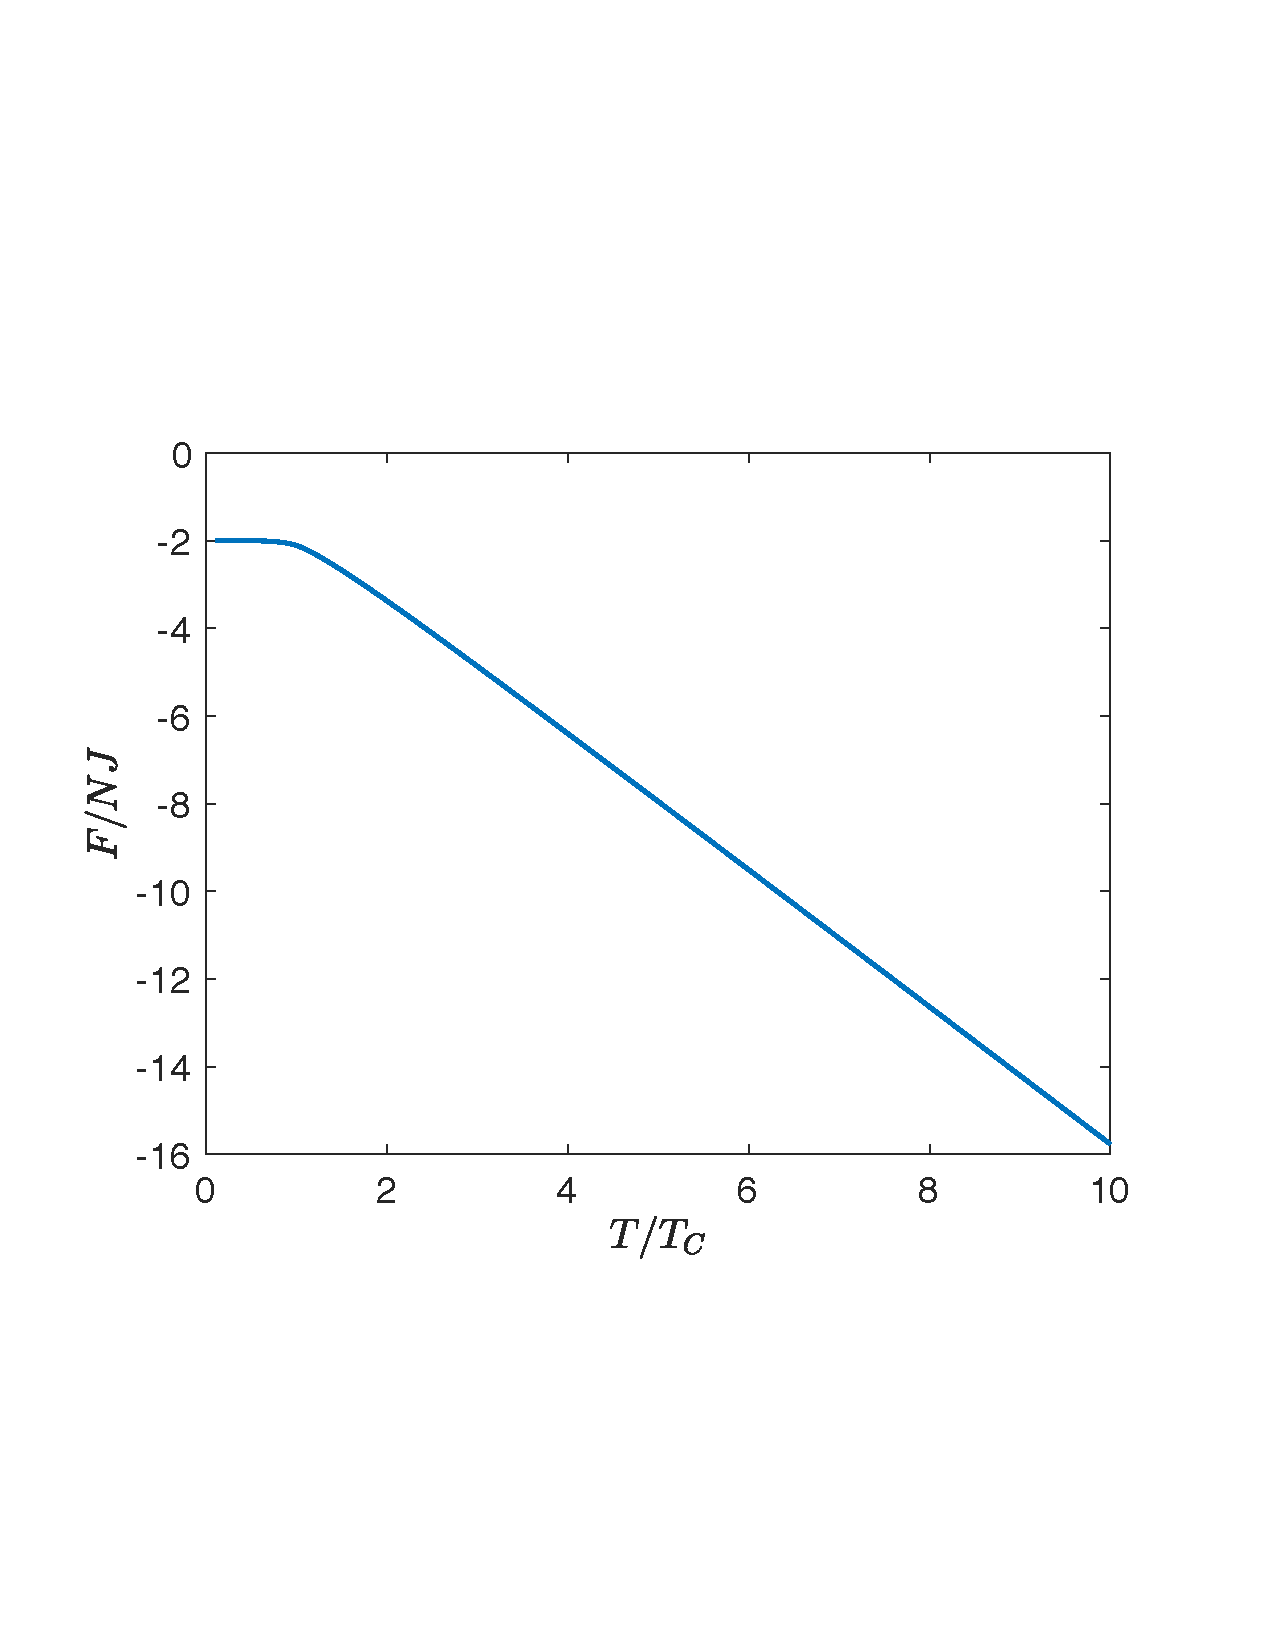
\includegraphics[width=10cm]{ising_free_energy}
\caption{{\it Free energy of the 2D Ising model.}}
\end{center}
\end{figure}
%
The free energy is related to the entropy and internal energy through
%
\begin{align*}
F &= U -T S\;.
\end{align*}
%
As we will easily see later on, for $T\to 0$ we have $U\to -2 J N$
and $S\to 0$  (3. law of thermodynamics), hence $F\to -2 J N$;
while for $k_{B}T/J \gg 1$ we have $U\to 0$
and $S\to N k_{B} \ln(2)$, hence $F\to - N k_{B} T \ln(2)$.

\subsection{Curie-temperature}

If we would have computed the free energy in the presence of an external magnetic field,
we could have computed the magnetization  and from that directly the transition temperature. 
In the absence of an external field, the magnetization is always zero, due to symmetry.
But in order to allow for a  phase transition the free energy has to have an irregularity.
(The argument will be given later.)
The argument of the logarithm is non-negative, but it can be zero which yields the required irregularity.
For the argument to become zero, both terms $(1-\sinh(2j))^{2}$ and $\sinh(2j)(2+\varepsilon)$ have to be zero.
The first condition yields
%
\begin{align}\label{eq:jC:2d:ising}
\sinh(2 j_{C}) &=1 
\end{align}
%
%
\begin{align*}
1 -\sinh(2j) &=  1 - \frac{e^{2j_{C}}+e^{-2j_{C}}}{2} = 0\\
\Rightarrow\qquad e^{2j_{C}}+e^{-2j_{C}} -2 &=0\\
e^{4j_{C}} -2 e^{2j_{C}} + 1&=0\;.
\end{align*}
%
This quadratic equation has the solutions
%
\begin{align*}
e^{2j_{C}} &= 1 \pm\sqrt{2}\;.
\end{align*}
%
Since $e^{2j}>0$ the only solution is 
%
\begin{align}\label{eq:}
j_{C} = J \beta_{C} &= \frac{1}{2}\ln\big( 1+\sqrt{2} \big) = 0.4407\;.
\end{align}
%
\blue{The mean field result was $J \beta_{C} = 0.25$.}
The irregularity  of the free energy is a necessary prerequisite for phase transition, but not 
sufficient for a rigorous prove. Nor does it tell us the order of the phase transition.
The rigorous prove requires the dependence of the free energy on the an external field.
\newpage

\subsection{Internal energy}
%
\begin{align*}
U &= \langle H \rangle = -J\sum_{\langle ij \rangle} \langle S_{i}S_{j}\rangle\;.
\end{align*}
%
Due to the translational invariance all n.n. correlations are
the same
\begin{align*}
\frac{U}{NJ} &=-2 \langle S_{1}S_{2}\rangle\;.
\end{align*}
For high temperatures the spins are uncorrelated resulting in
\begin{align*}
\frac{U}{NJ} &=-2 \langle S_{1}\rangle \langle  S_{2}\rangle = 0\;,
\end{align*}
while for $T=0$, the lowest energy is obtained if all spins are parallel 
and
\begin{align*}
\frac{U}{NJ} &=-2\;.
\end{align*}
Now we compute $U$ for arbitrary temperature.
%
To this end, we write $\ln(Z)$ in a more compact form
%
\begin{align*}
\ln(Z) &= \ln(2) +\frac{1}{2} 
\underbrace{
\avg{\ln \bigg((1-\kappa)^{2} + \kappa (2+\varepsilon) \bigg)}
}_{\color{blue} = g(\kappa)}\;,
\end{align*}
%
the average here is taken w.r.t. $\rho(\varepsilon)$, and $\kappa=\sinh(2 \beta J)$. Then
\begin{align*}
\frac{U}{N} &= \frac{\langle H \rangle}{N} = -\frac{\partial \ln(Z)}{\partial \beta}\\
&=-\frac{1}{2} \big(\frac{\partial }{\partial \kappa} g(\kappa) \big)
\frac{d \kappa}{d\beta}\;.
\end{align*}
%
with
%
\begin{align*}
\frac{\partial \kappa}{\partial \beta}&= \frac{\partial }{\partial \beta} \sinh(2 J \beta) = 2 J \cosh(2 J \beta)= 2J \sqrt{ 1+\sinh^{2}(2 J\beta) }
\end{align*}
%
we have 
%
\begin{align*}
\frac{U}{N}&=-J g'(\kappa) 
\sqrt{1+\kappa^{2}} \\
&=-J \avg{
\frac{2\kappa +\varepsilon}{(1-\kappa)^{2}+\kappa(2+\varepsilon)}
}
\sqrt{1+\kappa^{2}} \;.
\end{align*}
%
In summary we have
%
\tboxit{Internal energy}{
\begin{align}\label{eq:ising:U}
\frac{U}{N J} &= -  \avg{
\frac{2\kappa +\varepsilon}{(1-\kappa)^{2}+\kappa(2+\varepsilon)}
}
\sqrt{1+\kappa^{2}} \;.
\end{align}}
%

%
\begin{figure}[t]
\subfigure[Internal energy .]{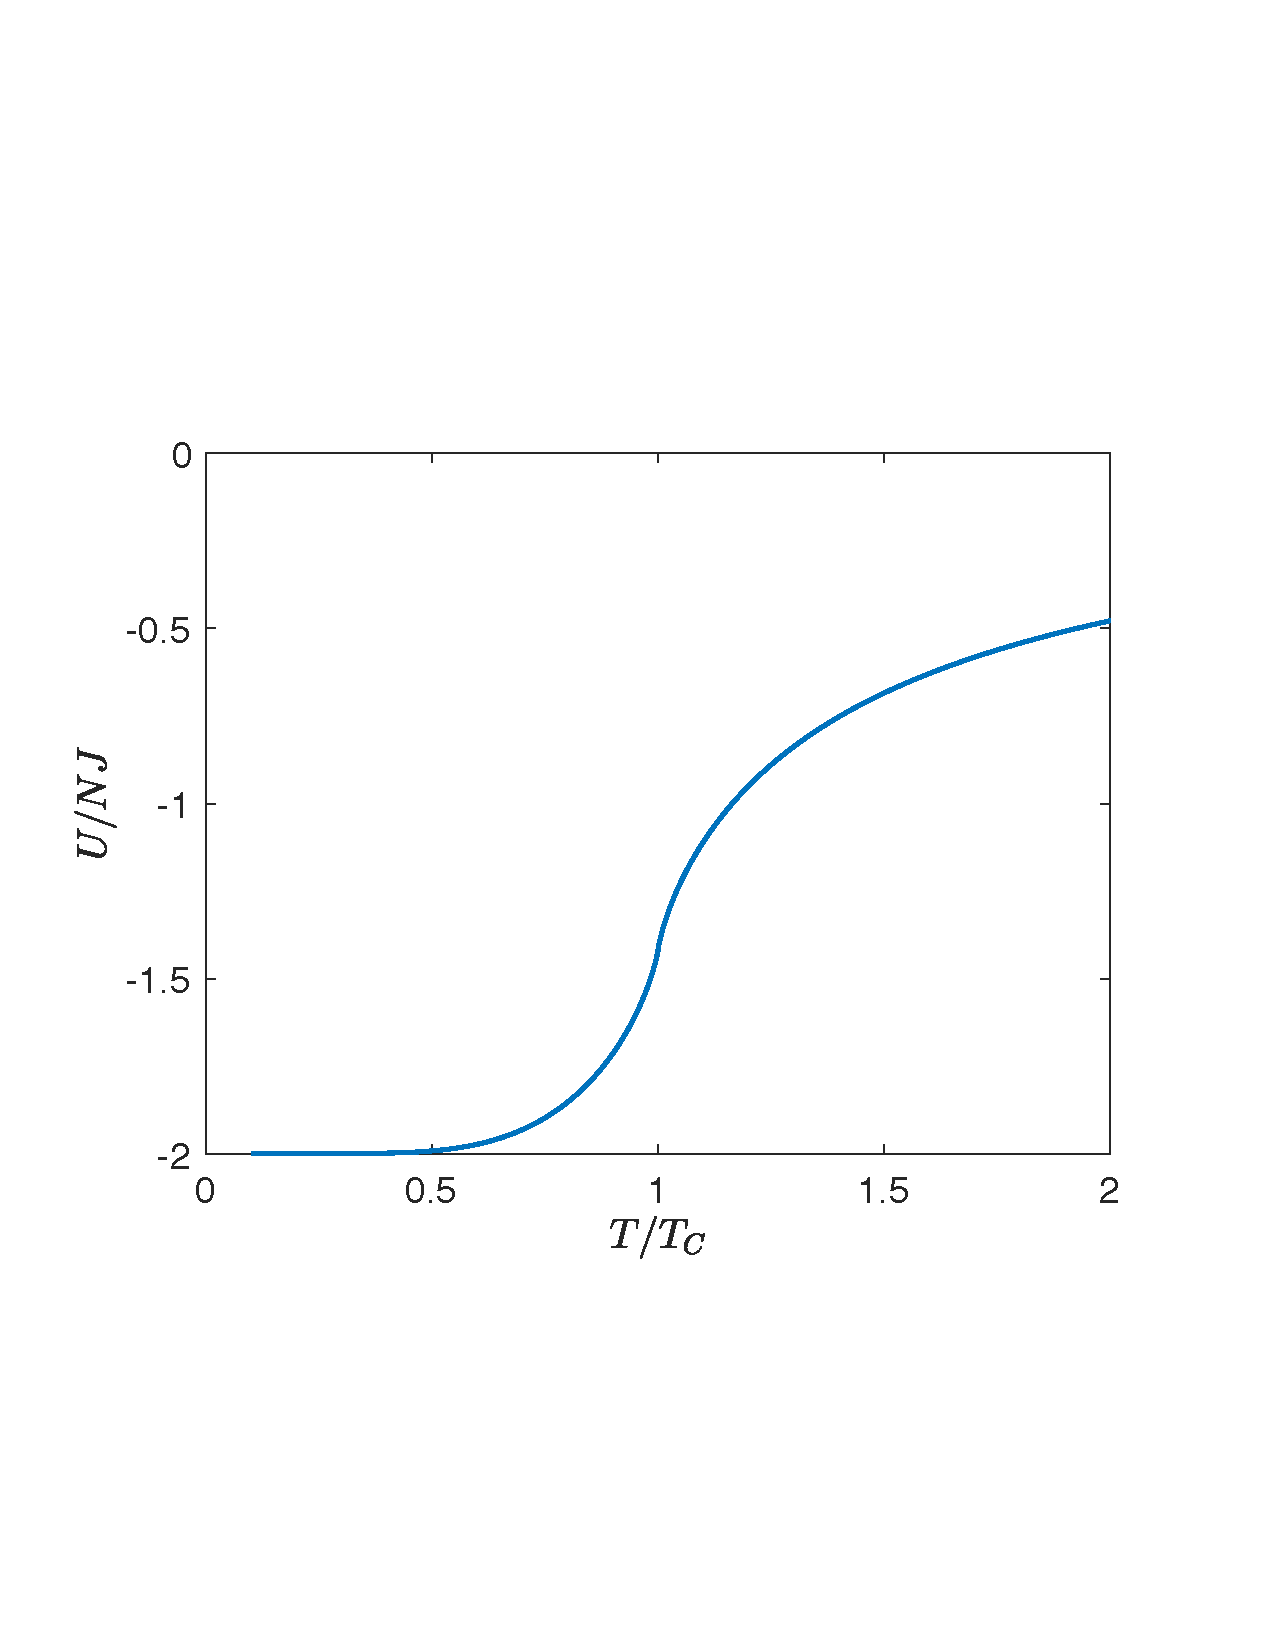
\includegraphics[width=0.53\textwidth]{ising_internal_energy}} 
\subfigure[Entropy.]{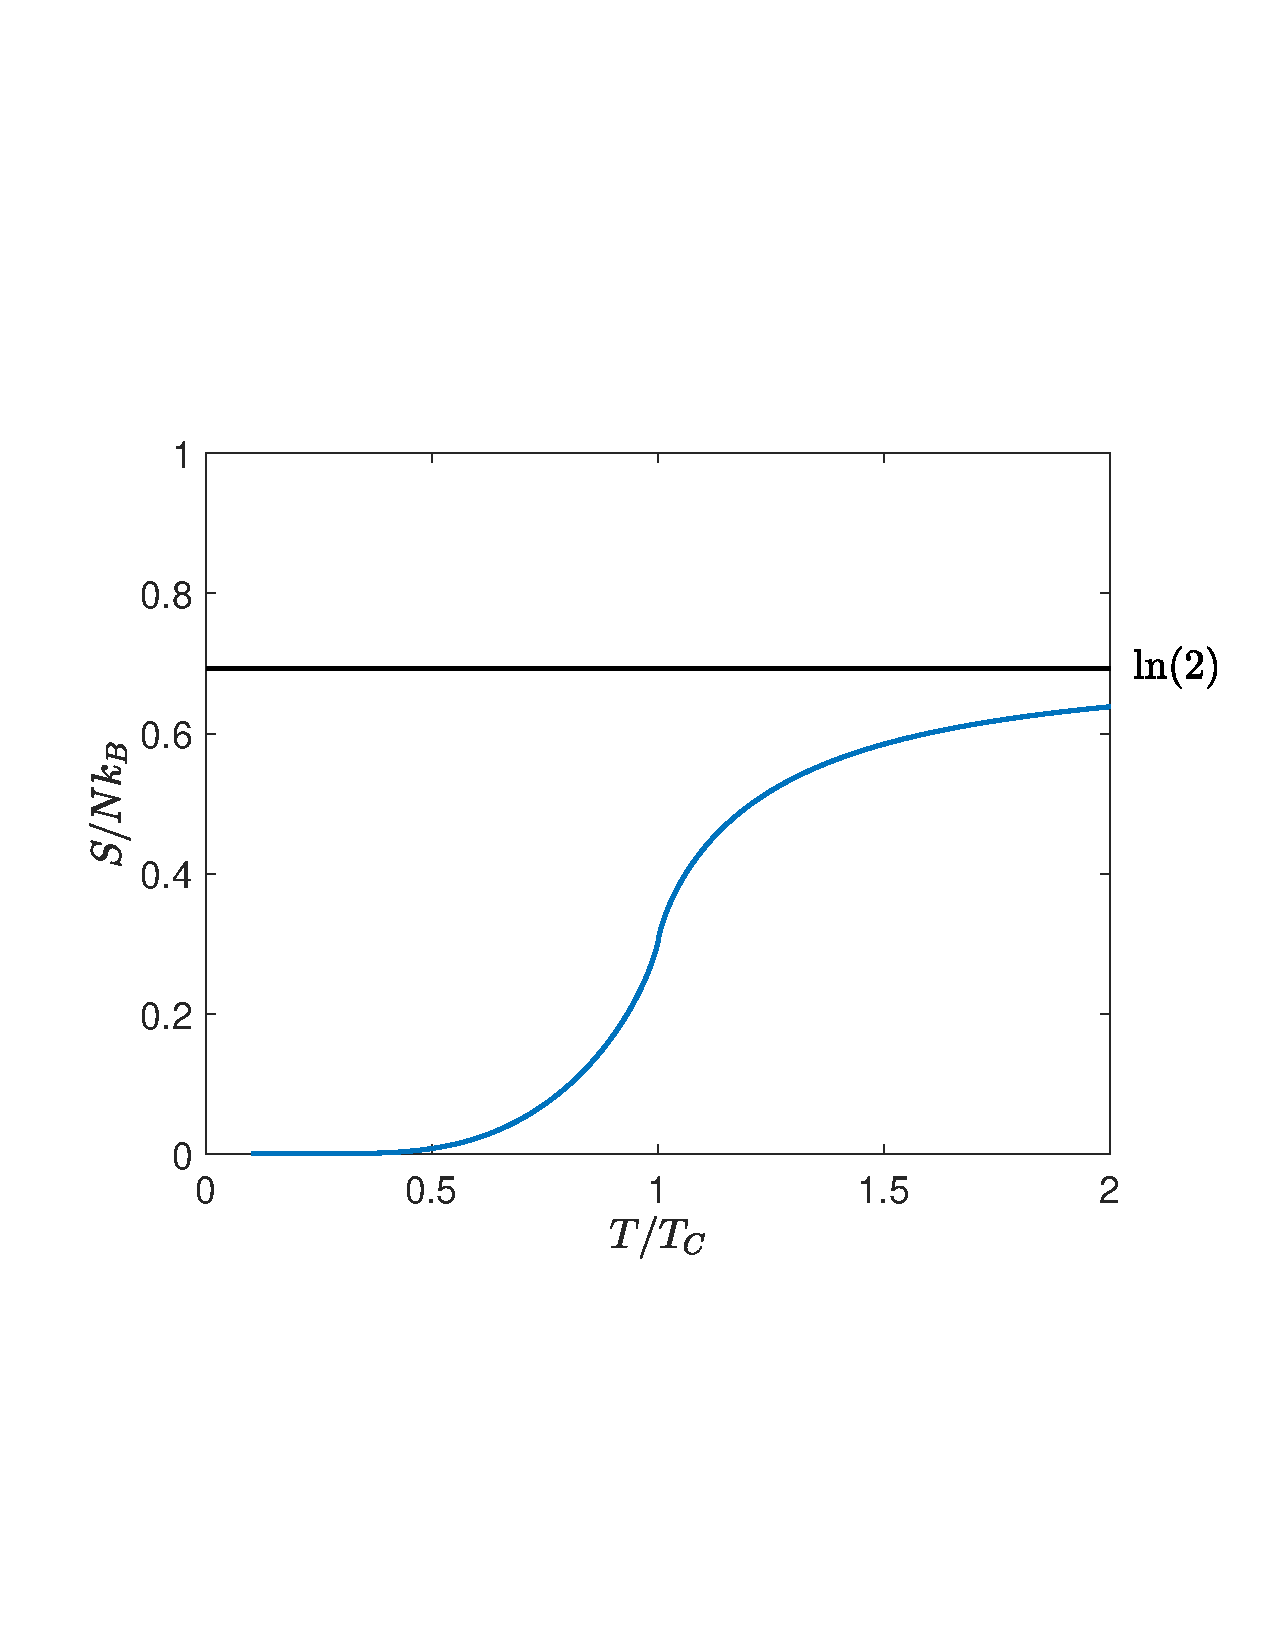
\includegraphics[width=0.55\textwidth]{ising_entropy}} 
\caption{{\it 2d Ising model for $B=0$.}\label{fig:graph:ising:int:energy}}
\end{figure}




\subsection{Entropy}
%
%

%

From $F=U-TS$ we get
\begin{align*}
\frac{S}{N k_{B}} &= j \frac{U}{N J} - \beta \frac{F}{N }
= j \bigg(\frac{U}{N J} \bigg)+\bigg( \frac{\ln(Z)}{N}\bigg)\;.
\end{align*}
%
Hence, we  can express the entropy in terms of \eq{eq:ising:U} and 
\eq{eq:ising:ln:Z}.


We see no critical behaviour in the entropy, which is   the first derivative of the free energy w.r.t. $T$. The latter is continuous at $T_{C}$. According to 
\SEC{sec:ehrenfest:classification} it is therefore not a first order phase transition.

\subsection{Specific heat \label{sec:Ising:2D:spec:heat}}

The order of the phase transition can also be inferred from the specific heat at $B=0$.
%
\begin{align*}
\frac{C}{N} &= \frac{1}{N}\pder{U}{T}{N} 
=\frac{1}{N} \frac{\partial U}{\partial \kappa} 
\underbrace{
\frac{\partial \kappa}{\partial \beta }
}_{\color{blue} =   2J \sqrt{1+\kappa^{2}} }
\underbrace{
\frac{\partial \beta}{\partial T}
}_{\color{blue} = -\frac{1}{k_{B}T^{2}} }\\
&= 
\bigg[\frac{\partial}{\partial \kappa}\bigg(- J g'(\kappa) \sqrt{1+\kappa^{2}} \bigg)\bigg]\;
\bigg(-k_{B}\beta^{2}\big( 2J \sqrt{1+\kappa^{2}} \big)  \bigg)
\end{align*}
%
The final result reads
%

\begin{subequations}\label{eq:spec:heat:2d:ising}
\begin{align}
\frac{C(T)}{N k_{B}}&= 2 j^{2}\;\bigg[\big(1+\kappa^{2} \big)  
 g''(\kappa) + \kappa g'(\kappa) \bigg]\;.
%
\intertext{with}
%
g'(\kappa) &=
\avg{
\frac{2\kappa +\varepsilon}{(1-\kappa)^{2}+\kappa(2+\varepsilon)}
}\\
g''(\kappa) &=
\avg{
\frac{2}{(1-\kappa)^{2}+\kappa(2+\varepsilon)}
}
-
\avg{
\bigg(\frac{2\kappa +\varepsilon}{(1-\kappa)^{2}+\kappa(2+\varepsilon)}\bigg)^{2}
}
\end{align}
\end{subequations}
%
We see in \fig{fig:spec:heat:2d:ising} that the specific heat diverges at $T_{C}$.
In order to unravel the type of divergency we perform a Taylor expansion
in $T$ about $T_{C}$, i.e. $T = T_{C}+\Delta T$. This corresponds to
%
\begin{align*}
j &=j_{C} + \Delta j\\
\kappa &=\sinh(2 J_{C}) + \Delta \kappa = 1  +  \Delta \kappa 
\end{align*}
%
In the last step we have used \eq{eq:jC:2d:ising}.
%
The only divergent behaviour  can come from $g'$ or $g''$.
The other terms can, therefore,  be replaced by $T=T_{C}$. I.e.
\begin{align*}
\frac{C(T_{C}+\Delta T)}{N k_{B}}&= 2 j_{C}^{2}\;
\big[2  g''(\kappa_{c}+\Delta\kappa) + g'(\kappa_{c}+\Delta\kappa) \big]\;.
\end{align*}
%
\begin{figure}[t]
\begin{center}
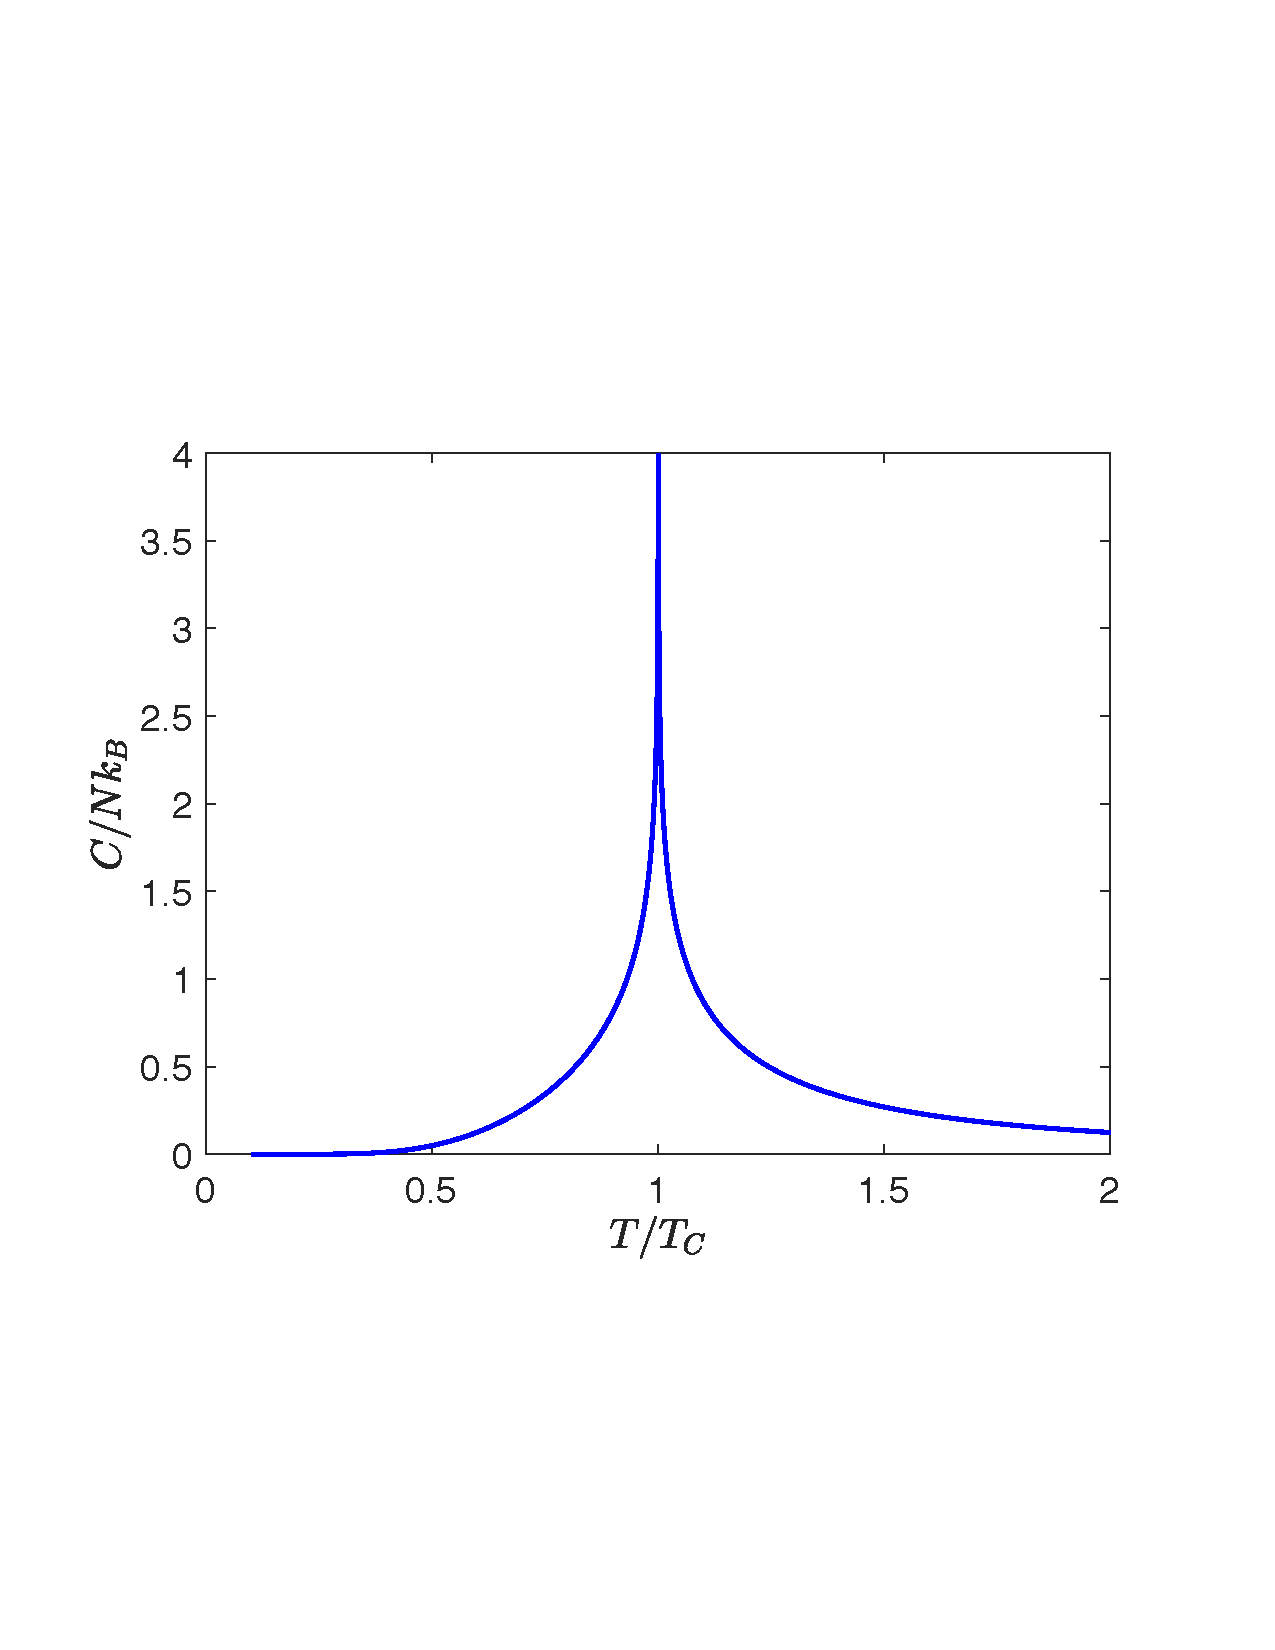
\includegraphics[width=9cm]{ising_spec_heat}
\caption{{\it Specific heat of the 2d Ising model.\label{fig:spec:heat:2d:ising}}}
\end{center}
\end{figure}
There is a critical behaviour in the second derivative of $F$, i.e. the specific heat. Therefore, the Ising model has \blue{a second order phase transition}.
\newpage

\subsubsection{Type of divergency}
The divergency originates from the term $\frac{1}{(1-\kappa)^{2}+\kappa(\varepsilon+2)}$ at the vicinity of  $\varepsilon=-2$.
The dos $\rho(\varepsilon)$ in principle also has a divergency at $\varepsilon=0$ but it is integrable and does not result in a divergence
in the specific heat.
To study the divergency at $\varepsilon=-2$ we split 
%
\begin{align*}
\rho(\varepsilon) &= \underbrace{
\rho(-2)
}_{\color{blue} = \rho_{0}}  + \Delta \rho(\varepsilon)\;.
\end{align*}
%
Then the expectation values become
%
\begin{align*}
\avg{F(\varepsilon)} &= \avg{F(\varepsilon)}_{\rho_{0}} + 
\avg{F(\varepsilon)}_{\Delta\rho}\;.
\end{align*}
%
The second term cause no divergency, hence  we merely need to consider terms of the form
%
\begin{align}\label{eq:}
\avg{F(\varepsilon)}_{\rho_{0}}\;.
\end{align}
%
\emphasize{Proof}{
%
\begin{align*}
&\lim_{\varepsilon\to -2} \frac{\Delta \rho(\varepsilon)(2+\varepsilon +2 \Delta\kappa)}{(\Delta\kappa)^{2} + (1+\Delta\kappa)\big(\varepsilon+2\big)} \\
&=\lim_{\eta\to 0} \frac{\Delta \rho(-2+\eta )(\eta +2 \Delta\kappa)}{(\Delta\kappa)^{2} + (1+\Delta\kappa)\eta} \\
&\overset{\text{L'Hospital}}{=}\lim_{\eta\to 0}  \frac{\Delta \rho'(-2+\eta )(\eta +2 \Delta\kappa) + \Delta\rho(-2+\eta)  }{(\Delta\kappa)^{2} + (1+\Delta\kappa)\eta} \\
&= \lim_{\eta\to 0}  \frac{(2 \Delta\kappa \Delta \rho'(-2+\eta ) + \Delta\rho(-2+\eta)  }{(\Delta\kappa)^{2} } \\
&= \frac{2}{\Delta\kappa}\underbrace{
 \lim_{\eta\to 0} \Delta \rho'(-2+\eta )
}_{\color{blue} = 0} +  \frac{1 }{(\Delta\kappa)^{2} }  \underbrace{
\lim_{\eta\to 0}  \Delta\rho(-2+\eta) 
}_{\color{blue} = 0}\\
&= 0\;.
\end{align*}
% 
or for $g''$ we need
%
\begin{align*}
&\lim_{\varepsilon\to -2} \Delta \rho(\varepsilon) \bigg(\frac{2+\varepsilon+\Delta\kappa}{\big(\Delta \kappa\big)^{2} + (1+\Delta\kappa) \big(\varepsilon+2\big)}\bigg)^{2}\\
&=\lim_{\eta\to 0}  \frac{\Delta \rho(-2+\eta ) \big(\eta+\Delta\kappa\big)^{2}}{\big(\big(\Delta \kappa\big)^{2} + (1+\Delta\kappa) \eta\big)^{2}}\\
&\overset{L'Hospital}{=}\lim_{\eta\to 0}  \frac{\Delta \rho'(-2+\eta ) \big(\eta+\Delta\kappa\big)^{2}+ 2\Delta \rho(-2+\eta ) \big(\eta+\Delta\kappa\big)}
{2 \big(\big(\Delta \kappa\big)^{2} + (1+\Delta\kappa) \eta\big)\big( 1+\Delta\kappa \big)}\\
&\overset{L'Hospital}{=}\lim_{\eta\to 0}  \frac{\Delta \rho'(-2+\eta ) \big(\Delta\kappa\big)^{2}+ 2\Delta \kappa \Delta \rho(-2+\eta ) }
{2 \big(\big(\Delta \kappa\big)^{2} \big)\big( 1+\Delta\kappa \big)}\\
&=
\frac{ \big(\Delta\kappa\big)^{2}}
{2 \big(\big(\Delta \kappa\big)^{2} \big)\big( 1+\Delta\kappa \big)}
\underbrace{
\lim_{\eta\to 0}  \Delta \rho'(-2+\eta ) 
}_{\color{blue} = 0}
+\frac{ 2\Delta \kappa}
{2 \big(\big(\Delta \kappa\big)^{2} \big)\big( 1+\Delta\kappa \big)}\underbrace{
\lim_{\eta\to 0}  \Delta \rho(-2+\eta )
}_{\color{blue} = 0} \\
&=0\;.
\end{align*}}
%
%% end of proof
% 
For the first term in \eq{eq:spec:heat:2d:ising} we need
%
\begin{align*}
g'(1+\Delta\kappa) &= \avg{\frac{\varepsilon+2+\Delta\kappa}{
(2+\varepsilon)( 1+\Delta\kappa ) +(\Delta\kappa)^{2} }}_{\rho_{0}}\;,
\end{align*}
%
for which we find
\begin{align*}
g'(1+\Delta\kappa) 
&=\frac{1}{1+\Delta\kappa} \cdot 
\left\{
4 \rho_{0} + \Delta\kappa  \rho_{0} \ln\big( 4 \big) - 2 \rho_{0} \Delta\kappa \ln\big( \Delta\kappa \big )  + O\big(\Delta\kappa\big)
\right\}\\
&\underset{\Delta\kappa \to 0}     {\longrightarrow} 4\rho_{0} = O(1)\;.
\end{align*}
\emphasize{Proof}{
First we will transform the denominator 
%
\begin{align*}
(2+\varepsilon)( 1+\Delta\kappa ) +(\Delta\kappa)^{2}  &=
( 1+\Delta\kappa )  \bigg(2+\varepsilon+\frac{(\Delta\kappa)^{2}}{1 +\Delta\kappa} \bigg)\\
&= ( 1+\Delta\kappa )  \bigg(2+\varepsilon+ (\Delta\kappa)^{2} + O((\Delta\kappa)^{3})\bigg)\\
\end{align*}
Then
%
\begin{align*}
&\frac{\varepsilon+2+\Delta\kappa}{
(2+\varepsilon)( 1+\Delta\kappa ) +(\Delta\kappa)^{2} } \\
&=\frac{1}{1+\Delta\kappa} \cdot 
\frac{\varepsilon+2+\Delta\kappa}{2+\varepsilon+ (\Delta\kappa)^{2} + O((\Delta\kappa)^{3}}\\
&=\frac{1}{1+\Delta\kappa} \cdot 
\frac{\varepsilon+2+(\Delta\kappa)^{2} + O((\Delta\kappa)^{3}) + \Delta\kappa\big( 1-\Delta\kappa \big)   +O((\Delta\kappa)^{3})  }{2+\varepsilon+ (\Delta\kappa)^{2} + O((\Delta\kappa)^{3})}\;.
\end{align*}
%
I.e.
%
\begin{align}\label{eq:aux:a}
\frac{\varepsilon+2+\Delta\kappa}{
(2+\varepsilon)( 1+\Delta\kappa ) +(\Delta\kappa)^{2} } 
&=\frac{1}{1+\Delta\kappa} \cdot 
\left\{ 1 + \frac{ \Delta\kappa\big( 1-O\big((\Delta\kappa)^{2}\big) \big)   }{2+\varepsilon+ (\Delta\kappa)^{2}\big(1 + O(\Delta\kappa)\big)}\right\}\;.
\end{align}
%
So we have
%
\begin{align*}
&g'(1+\Delta\kappa) = \avg{\frac{\varepsilon+2+\Delta\kappa}{
(2+\varepsilon)( 1+\Delta\kappa ) +(\Delta\kappa)^{2} }}_{\rho_{0}}\\
&=\frac{1}{1+\Delta\kappa} \cdot 
\left\{\avg{1}_{\rho_{0}} + 
\Delta\kappa\big( 1-O\big((\Delta\kappa)^{2}\big) \big) \avg{\frac{1}{2+\varepsilon+ (\Delta\kappa)^{2}\big(1 + O(\Delta\kappa)\big)}}_{\rho_{0}}\right\}\\
\end{align*}
%
The definition of the expectation value is
%
\begin{align*}
\avg{f(\varepsilon)}_{\rho_{0}} &:= \int_{-2}^{2} f(\varepsilon) \rho_{0} d\varepsilon\;
= \rho_{0}\int_{-2}^{2} f(\varepsilon) d\varepsilon\;.
\end{align*}
%
Therefore
%
\begin{align*}
\avg{1}_{\rho_{0}} &= 4 \rho_{0}\;.
\end{align*}
%
%
\begin{align*}
& \avg{\frac{1}{2+\varepsilon+ (\Delta\kappa)^{2}\big(1 + O(\Delta\kappa)\big)}}_{\rho_{0}}\\&=
 \rho_{0}
\int_{-2}^{2}
\frac{1}{2+\varepsilon+ (\Delta\kappa)^{2}\big(1 + O(\Delta\kappa)\big)} d\varepsilon\\
&=\rho_{0} \ln\bigg( 2+2+(\Delta\kappa)^{2}\big(1 + O(\Delta\kappa)\big) \bigg)
-\rho_{0} \ln\bigg( 2-2+(\Delta\kappa)^{2}\big(1 + O(\Delta\kappa)\big) \bigg)\\
&=\rho_{0} \ln\big( 4\big) 
-\rho_{0} \ln\big( \Delta\kappa)^{2}\big)  + O\big(\Delta\kappa\big)
\end{align*}
%
In total we have
%
\begin{align*}
&g'(1+\Delta\kappa) = \avg{\frac{\varepsilon+2+\Delta\kappa}{
(2+\varepsilon)( 1+\Delta\kappa ) +(\Delta\kappa)^{2} }}_{\rho_{0}}\\
&=\frac{1}{1+\Delta\kappa} \cdot 
\left\{
4 \rho_{0} + \Delta\kappa  \rho_{0} \ln\big( 4 \big) - 2 \rho_{0} \Delta\kappa \ln\big( \Delta\kappa \big )  + O\big(\Delta\kappa\big)
\right\}\\
&\underset{\Delta\kappa \to 0}     {\longrightarrow} 0\;.
\end{align*}
}
%
% end oif proof

Similarly, for the second term of $g''$ we  find with \eq{eq:aux:a}
%
\begin{align*}
&\avg{
\bigg(\frac{2\kappa +\varepsilon}{(1-\kappa)^{2}+\kappa(2+\varepsilon)}\bigg)^{2}
}_{\rho_{0}}\\
 &= \bigg(\frac{1}{1+\Delta\kappa} \bigg)^{2}\cdot 
\avg{\bigg(1 + \frac{ \Delta\kappa\big( 1-O\big((\Delta\kappa)^{2}\big) \big)   }{2+\varepsilon+ (\Delta\kappa)^{2}\big(1 + O(\Delta\kappa)\big)}\bigg)^{2}}_{\rho_{0}}\\
&= O(1) + O(\Delta\kappa \ln(\Delta\kappa)) + O\big(\big(\Delta\kappa\big)^{2}\big)\int_{-2}^{2} \frac{1}{2+\varepsilon+\big(\Delta\kappa  \big)^{2}}d\varepsilon\\
&= O(1) + O(\Delta\kappa \ln(\Delta\kappa)) + O\big(\big(\Delta\kappa\big)^{2}\big)
\bigg( O(1) + O\big( \frac{1}{(\Delta\kappa)^{2}} \big) \bigg)\\
&=  O(\Delta\kappa \ln(\Delta\kappa))+O(1) + O(\big( (\Delta\kappa)^{2} \big)
\end{align*}
%
Again no divergency.
The only divergent term stems from the first part of $g''$, which yields
%
\begin{align*}
&\avg{\frac{2}{(\Delta\kappa)^{2}+(1+\Delta\kappa)(2+\varepsilon)}}_{\rho_{0}} 
=
\int_{-2}^{2} \frac{\rho_{0} }{(\Delta\kappa)^{2}+(1+\Delta\kappa)(2+\varepsilon)} d\varepsilon\\
&= \rho_{0} \ln\big[ (\Delta\kappa)^{2}+(1+\Delta\kappa)(2+2) \big]
-
\rho_{0} \ln\big[ (\Delta\kappa)^{2}+(1+\Delta\kappa)(2-2) \big]\\
&= \rho_{0} \ln\big[ 4 + O\big(\Delta\kappa\big) \big]
-
2 \rho_{0} \;\ln(\abs{\Delta\kappa});\\
&=O(1)  - 2 \;\ln(\abs{\Delta\kappa});
\end{align*}
%
The specific heat obviously has a logarithmic divergency, which corresponds
to the critical exponent
%
\begin{align}
\alpha &=\alpha' = 0\;.
\end{align}
%
For the definition of the critical exponents see \SEC{sec:critical:exponents}.

%
\subsection{Spontaneous magnetization}
So far it has not been possible to find the exact solution of the 2d Ising model in an external magnetic
field. This is only doable for infinitesimal $B$ values, which is enough to determine the spontaneous 
magnetization. It amounts to computing the spin-spin correlation $\langle S_{i} S_{j}\rangle$ and use
%
\begin{align*}
\lim_{l\to\infty} \langle S_{i}  S_{i+l}\rangle \longrightarrow \bigg(  \langle S_{i} \rangle\bigg)^{2}
= \bigg(\frac{M}{N }\bigg)^{2}\;.
\end{align*}
%
The graphical solution amounts to count all graphs as before but with the peculiarity that 
the vertices $i$ and $j$ have an odd order.
The result reads
\tboxit{Spontaneous Magnetization of the 2d Ising Model}{
%
\begin{align}\label{eq:}
\frac{M}{N}&=
\begin{cases}
	\big( 1-\sinh^{-4}(2 j) \big)^{1/8}&\text{for } T\le T_{C}\\
	0&\text{otherwise}
\end{cases}
\end{align}
%
}
The order parameter, the magnetization, is continuous, which corroborates 
the statement, that it is a second order phase transition.
%
\begin{figure}[t]
\begin{center}
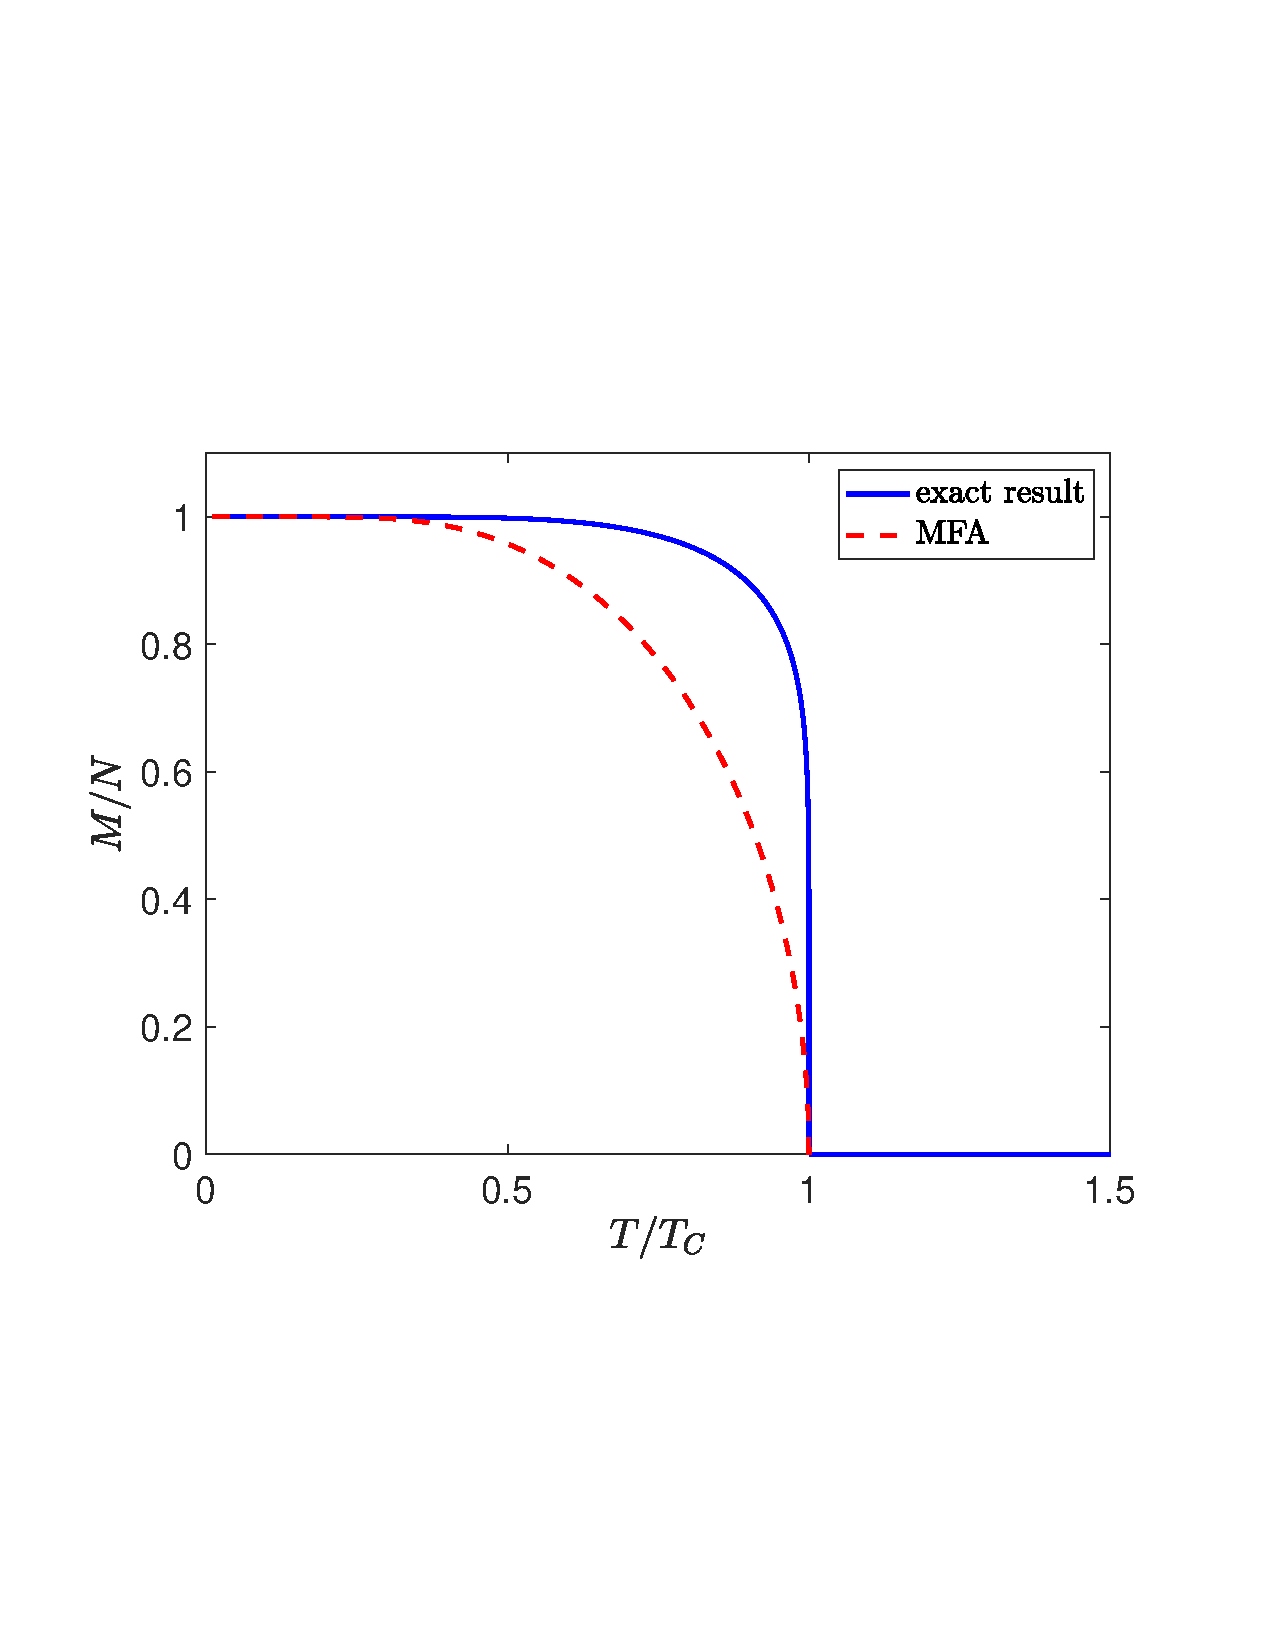
\includegraphics[width=9cm]{ising_magnetization}
\caption{{\it Spontaneous magnetization of Ising spins.}}
\end{center}
\end{figure}
%

%
\subsection{Proof}

We seek the number of paths from the center $\vv x=0$ to site $\vv x$, where the Manhattan distance is 
$n$. We consider only cases with $n>1$, actually we are interested in $n-1$ to $\infty$. 
We are interested in the weighted sum over all paths from the center to site $\vv x$. Schematically this can be written as
%
\begin{align*}
Z_{0 \vv x} &= \sum_{m=n}^{\infty}  W^{(m)}_{0,\vv x}\;,
\end{align*}
%
where $W^{(m)}_{0,\vv x}$ stands for the contributions that contain $m$ steps. We will again use the previous matrix $M^{(m)}$. Here, however, we are not counting loops and therefore the weights are not entirely correct
and it is not yet clear what we have to do with the directions of the last step, which points from the final point $\vv x$ to an arbitrary direction. It is, therefore, useful, to split off the last step. Then it seem reasonable to 
start with the form
%
\begin{align*}
W^{(m)}_{0,\vv x} &= \sum_{\vv d_{0}} \sum_{\vv x',\vv d'}  \bigg(M^{(m-1})\bigg)_{(\vv 0,\vv d_{0}),(\vv x',\vv d')}  \big(M^{(1)}\big)_{(\vv x',\vv d'),(\vv x,\vv d'')}
\end{align*}
%
There is one constraint:
%
\begin{align*}
\vv x'  &= \vv x - \vv d'\;.
\end{align*}
%
The last term adds a factor $th(j)$ plus a phase, that depends on the yet undefined $\vv d''$.
The phase-factors are only correct in closed loops to add up to the sign, representing crossings.
Therefore, we will add graph elements to from a closed loop, such that no additional crossings occur.
There are 16 possibilities depending on $\vv d$ and $\\vv d'$
%
%\begin{table}[]
%\begin{tabular}{llllll}
% 1)&  $\vv d = \$  & i.e. a loop is closed  &$\Rightarrow$ &   $f= Straight$  \\
% 2)&  $\vv d'= -\vv d = \vv e \alpha$  & i.e. a loop is closed  &$\Rightarrow$ &   $f= 2 left$  \\
%  3)&  $\vv d'= -\vv d = -\vv e \alpha$  & i.e. a loop is closed  &$\Rightarrow$ &   $f= 2 right$  \\
%   4)&  $\vv d'= -\vv d = \vv e x$  & i.e. a loop is closed  &$\Rightarrow$ &   $f= LL$  \\
% &  &  &  &  \\
% &  &  &  & 
%\end{tabular}
%\end{table}
%
%
%
%kerze


\subsection{Critical exponent \label{sec:Ising:2D:beta}}
For  $T\searrow T_{C}$ we have
%
\begin{align*}
\frac{M}{N} &= \bigg( 1 - \big[\sinh\big( 2 j_{C} + 2J\Delta \beta  \big)\big]^{-4} \bigg)^{\frac{1}{8}}\\
&= \bigg( 1 - \underbrace{
\big[\sinh\big( 2 j_{C}\big)
}_{\color{blue} \overset{(\ref{eq:jC:2d:ising})}{=} 1} + \cosh\big(2j_{C}  \big) J\Delta \beta\big]^{-4} \bigg)^{\frac{1}{8}}\;.
\end{align*}
%
In addition, we have 
%
\begin{align*}
\cosh\big( 2 j_{C} \big) &= \sqrt{1+\sinh^{2}(2 j_{C})} = \sqrt{2}\;.
\end{align*}
%
Hence
%
\begin{align*}
\frac{M}{N} &=\bigg( 1 - \big[ 1 + \sqrt{2} J \Delta\beta \big]^{-4} \bigg)^{\frac{1}{8}}\\
&=\bigg( 1 - 1 +4\sqrt{2}  J \Delta\beta  \bigg)^{\frac{1}{8}}\\
&=\bigg(4\sqrt{2}  J \Delta\beta  \bigg)^{\frac{1}{8}}\\
&=\propto  \big(\frac{1}{T}-\frac{1}{T_{C}}\big)   ^{\frac{1}{8}}\\
&\propto \varepsilon^{\frac{1}{8}}
\end{align*}
%


